\documentclass{article}
\usepackage[utf8]{inputenc}
\usepackage{comment}
\usepackage{duomasterforside}
\usepackage{listings}
\usepackage{float}
\usepackage{fancyvrb}
\usepackage{listings}
\usepackage{xcolor}
\usepackage{fvextra}
\usepackage{soul}
\usepackage{minted}
\usepackage{amssymb}
\usepackage{pifont}
\usepackage{multirow}
\graphicspath{ {./graphics/} }
\usepackage[backend=biber,natbib,style=numeric]{biblatex}
\usepackage{hyperref}
\addbibresource{references.bib}


\begin{document}

\title{Mobile Assets in Semantic Digital Twins}
\author{Oscar Lund Ramstad}
\date{January 2023}

\duoforside[dept={Institute for Informatics}, program={Informatics: Programming and System Architecture}, short]

\section*{Abstract}
This thesis proposes a solution to the challenge of handling mobile assets in a semantic digital twin based on a dynamic asset model in which static data (existing building infrastructure) is separated from dynamic data (smartphone's physical location). The digital twin (DT) is created in Semantic Micro Object Language (SMOL) for easy integration with semantic technologies, such as semantic knowledge graphs. In order to semantically enrich the DT further, a model of a building is created in Web Ontology Language (OWL). A hybrid smartphone application is implemented having the mobile assets in mind, which sends their updated status. The privacy of the data subjects is protected as much as possible. The DT is an up-to-date digital representation of the PT, and it reconfigures in near real-time if the PT or any of the mobile assets inside it changes. If a person is located inside a dangerous area, the app warns the appropriate user from the informed decision sent by the DT.


\newpage

\section*{Acknowledgements}
I would like to extend my greatest gratitude to those that helped me with this thesis. Thanks to Einar Broch Johnsen, Rudolf Schlatte, and Eduard Kamburjan for formidable guidance in writing this thesis. Einar, thanks for believing in me from the start. I have learned a lot from the discussions on separating the static analysis from the dynamic snapshots. Rudi, I have thoroughly enjoyed our many discussions on relevant subjects to this thesis, especially about the building domain and privacy. Eduard, thanks for giving me great feedback on my writing and everything SMOL related.

Thanks to my family, and especially my parents, for being there for me no matter what. I could never have done this without any of you.      
\newpage

\tableofcontents
\newpage

\listoffigures
\newpage

\pagenumbering{arabic}
\setcounter{page}{1}

\section{Introduction}\label{sec:Introduction}
\subsection{Context}
A digital twin (DT) is a digital representation of some physical system, referred to as a physical twin (PT), that is twinned in near real-time by the DT in order to understand or control the PT \cite{grieves_digital_2017, kamburjan_digital_2022}. The twinning aims to be bidirectional meaning that the DT both observes the PT and communicates informed decisions back to it \cite{kamburjan_digital_2022, fuller_digital_2020}. The DT must continually adapt to correctly reflect its physical twin \cite{kamburjan_twinning-by-construction_2022}. This may pose a challenge if the PT contains mobile assets, such as smartphones. The number of smartphone users worldwide is at an all-time high \cite{petroc_taylor_number_2023}. They are important resources for a company and can change at any time \cite{marcheta_development_2022}. 

It is stated by \citeauthor{godager_concept_2021} that although BIM could serve as a basis for DTs by providing lots of relevant information, DTs should give even more context about the built environment, especially by monitoring assets from near real-time data. A lot of work goes into modeling physical assets in general \cite{waszak_let_2022}, and using BIM is also very costly due to frequent updates by maintainers \cite{hamledari_ifc-based_2018}.

 Knowledge graphs (i.e. using graphs to represent data from diverse sources \cite{hogan_introduction_2022, ryen_building_2022}) are used in the interconnection of various elements in DTs. Furthermore, instead of storing all related data in one place, \citeauthor{waszak_let_2022} propose storing static and dynamic data sources in different places and linking them.

There exist challenges in handling mobile assets. Some systems mainly focus on tracking mobile assets and the accuracy of their physical location \cite{marcheta_development_2022,akram_design_2021}. If we keep the company's assets in mind, such a system could be improved upon by better understanding and controlling asset behavior. 

Furthermore, there is existing research about using Building Information Modeling (BIM) with standard data formats, such as JSON or Resource Description Framework (RDF), to better define static building infrastructure \cite{pauwels_live_2023}. \citeauthor{pauwels_live_2023} proposes how, and to what extent, such data can be used in robot navigation. Although BIM can be used, by default it has some challenges regarding interoperability due to heterogeneous data \cite{dinis_bim_2022,godager_concept_2021}.

Handling mobile assets in a DT based on an \emph{asset model} (i.e. a file that contains an organized description of an asset's composition and properties \cite{kamburjan_twinning-by-construction_2022}) that is \emph{dynamic} is unexplored territory.

\subsection{Motivation}\label{subsec:Motivation}
Given the gap that exists in connecting tracking systems, asset models, and digital twins, there is still room for improvement. The problem is that there exist no systems that have a digital twin (DT) based on a dynamic asset model which can track an unlimited number of heterogeneous smartphones. In an attempt to formalize heterogeneous data and make it understood by computers, semantic web technologies should be used. More specifically, we aim to semantically enrich a model of a building to increase interoperability, as well as keep it inexpensive and easy to maintain.

We envision an extension of a \emph{semantic} digital twin (i.e. a digital twin that processes heterogeneous data from different sources in the domain into generally understandable information \cite{birgit_boss_digital_nodate}) that handles mobile assets, and is based on a dynamic asset model in which static data (existing building infrastructure) and dynamic data (smartphone's physical location) is separated. The DT will be able to track an unlimited number of mobile assets simultaneously. The DT will be formalized using semantic web technologies. In the knowledge graph, static data will be noted to be different than dynamic data as it is generated from a combination of the program state and the asset model. 

The asset model will be automatically reloaded by the system itself, or manually updated by an operator either offline (online version updated from local changes), or directly online in an ontology editor. This way the mobile assets are not only tracked, but the physical system containing them is twinned in near-real time as well. The DT will get sensor data from the PT, and then send informed decisions back to the PT.

\subsection{Problem statement}\label{subsec:ProblemStatement}
From the context of digital twins and an increasing number of smartphone users, as well as the motivation for improvement described in Section \ref{subsec:Motivation}, we present the following hypothesis (H):

\begin{itemize}
    \item[\textbf{H:}] We can handle mobile assets in a semantic digital twin with the use of a dynamic asset model of a simple building, in which dynamic data (smartphone's physical location) is automatically updated by a server and separated from static data (existing building infrastructure), and informed decisions are sent back to the physical twin.
\end{itemize}


In addition to this, we present the following three research questions which will guide this thesis:
\begin{itemize}
    \item[\textbf{RQ1:}]
    How to create a dynamic asset model of a simple building that is also extensible?
    \item [\textbf{RQ2:}] 
    How to enable bidirectional data flow between the PT and DT, such that the digital twin gets updated sensor data from mobile devices and sends informed decisions back?
    \item [\textbf{RQ3:}]
    How to separate dynamic data (smartphone's physical location) from static data (building infrastructure) in the asset model?
\end{itemize}

Having the aforementioned in mind, an overview of the main architectural components in this thesis is shown below in Figure \ref{fig:initial_components}.

\begin{figure}[H]
    \centering
    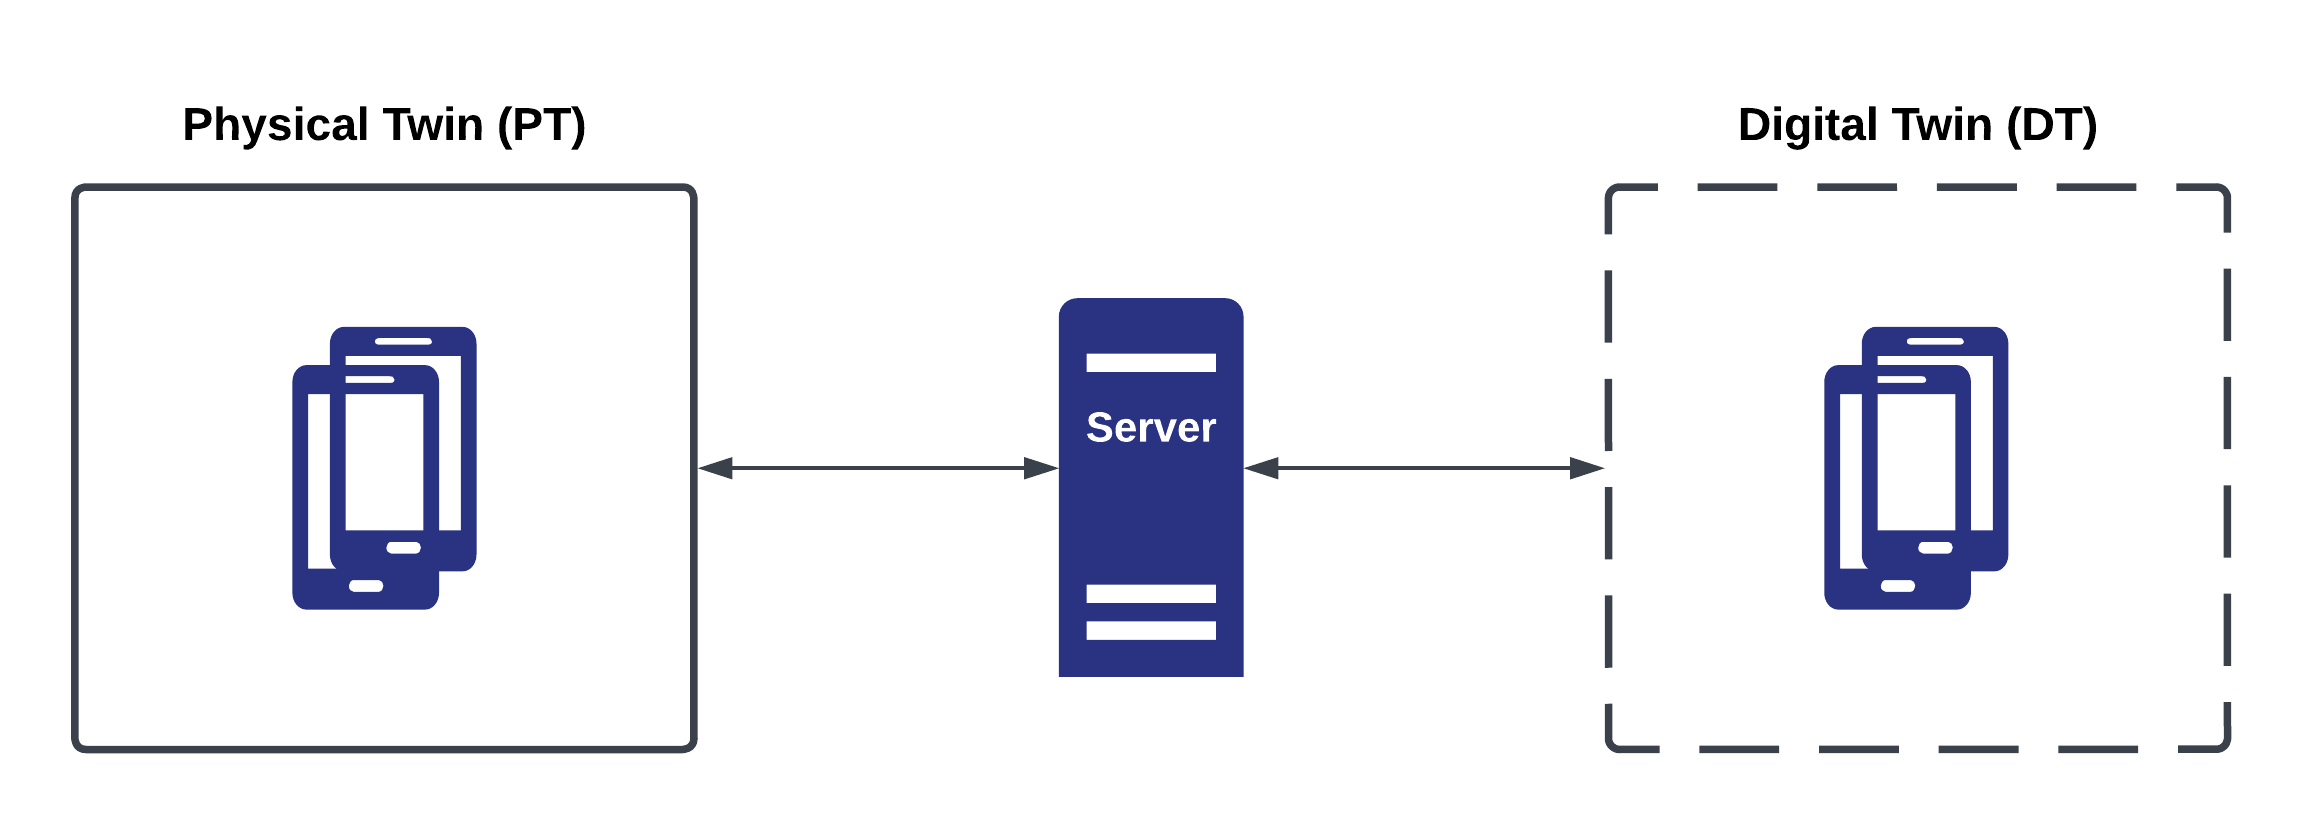
\includegraphics[scale=0.14]{graphics/initial_thesis_overview.png}
    \caption{Overview of \emph{main} architectural components in this thesis}
    \label{fig:initial_components}
\end{figure}


\subsection{Thesis scope and outline}\label{subsec:Scope}
The scope of this thesis is to handle an unlimited number of mobile assets in a semantic digital twin based on a dynamic asset model. Figure \ref{fig:initial_components} shows the overview of architectural components and the bidirectional data flow between the PT and DT. The digital twin should be developed using the Semantic Micro Object Language (SMOL) described in Section \ref{subsec:SMOL} and its publicly available interpreter\footnote{\url{https://github.com/smolang/SemanticObjects}}.

As noted by \citeauthor{pauwels_live_2023} many physical objects, such as furniture and doors, can be movable entities in a building apart from the robots. Doors will have one state (open). Laptops can also be considered mobile assets, but due to the context of a crisis situation, we are not able to justify adding support for it. We limit ourselves to smartphones and tablets in 2D space.  

The areas are predefined squares with latitude and longitude ranges, where we \emph{assume} the coordinates align. Square areas are easier to compute and scale into larger areas, and we are not concerned with other shapes such as polygons. The analysis of what certain area(s) are (e.g. what does a critical area mean) is also outside the scope of this thesis.

We are also assuming the PT contains a building in which there can be smartphones since we create a digital representation of a building in the DT.

Figure \ref{fig:simple_building} shows a simple building with two rooms connected by an inner wall with a door (open) in it.

\begin{figure}[H]
    \centering
    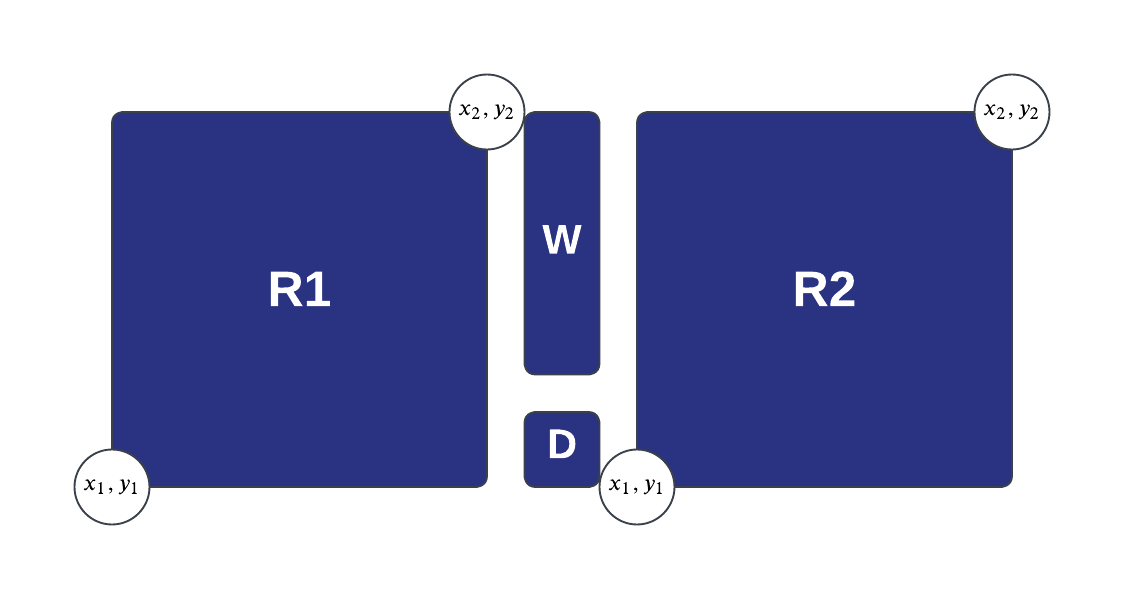
\includegraphics[scale=0.3]{graphics/simple_building.png}
    \caption{A simple building with the structural components: two rooms (R1 and R2) connected by an inner wall (W) with a door (D) in it}
    \label{fig:simple_building}
\end{figure}


The remainder of this thesis is organized as follows:
\begin{itemize}
    \item Chapter \ref{sec:Background} describes the theoretical background of this thesis.
    \item Chapter \ref{sec:Analysis} investigates the problem statement and the research questions. We also look at what a dynamic asset model means, as well as the separation of static and dynamic data.  
    \item Chapter \ref{sec:Implementation} dives into the implementation of the proposed solution and how the different architectural components shown in Figure \ref{fig:components} interact. More specifically, how do we "close the loop" by sending informed decisions back to the PT. 
    \item Chapter \ref{sec:Evaluation} evaluates the proposed solution according to the structural requirements that were set, and then according to various test runs.
    \item Chapter \ref{sec:Discussion} discusses the limitations of the discoveries in this thesis, the alternatives, and compares them to other existing work.
    \item Chapter \ref{sec:Conclusion} concludes this thesis and presents the contributions. We look at improvements that can be made to the proposed solution, and further work that can be done using the thesis as a basis.  
\end{itemize}



\newpage
\section{Background}\label{sec:Background}
This chapter describes the background information of this thesis. Starting off we give a description of digital twins (DTs). Then we give a description of the Semantic Web, as well as the technologies that help us build it. Later on we describe semantic reasoning and tools for it. Then we look at frameworks for building cross-platform applications from a single codebase. Near the end of the section, we describe real-time and time-series databases.

\subsection{Digital Twin}\label{subsec:DigitalTwins}
\subsubsection{Historic background}
The \emph{idea} of a digital twin can be traced back to the 1960s in NASA's space exploration days, where multiple simulations were employed to evaluate the problems with the space mission Apollo 13 \cite{noauthor_digital_nodate, fuller_digital_2020}. The \emph{term} digital twin was first introduced to the public by Michael Grieves in a presentation given in 2002, and in 2014 conceptualized as a virtual representation of a factory replication \cite{grieves_michael_digital_2014}. This set the foundation for developing digital twins \cite{grieves_michael_digital_2014, fuller_digital_2020}. Since then, DTs have had many applications in various disciplines, and in recent years especially in smart cities, healthcare, manufacturing, and asset management \cite{fuller_digital_2020, waszak_let_2022, macchi_exploring_2018}

\subsubsection{For the scope of this thesis}
As of today, a DT is referred to as a digital representation of some physical system \cite{grieves_digital_2017}, that has no restriction on the size or scale of it, which means the entity could be a single asset or a system of systems for that matter \cite{li_digital_2022, waszak_let_2022}. It exists in real life and is commonly referred to as the physical twin (PT), and is observed by the DT in near real-time. There should be a bidirectional flow of data between the DT and the PT throughout the life cycle of the PT. In other words, the DT gets updated sensor data from the PT, and sends informed decisions back to it \cite{madni_leveraging_2019, waszak_let_2022, kamburjan_digital_2022}. From this, and for the scope of this thesis, a DT is a digital representation of a system that tracks many mobile assets. The DT sends informed decisions to the physical counterpart in which the appropriate mobile assets perform actions.

There are multiple misconceptions about DTs. One such misconception is that a digital shadow (DS) is some sort of a DT. This misconception often leads people to build shadows instead of DTs. \cite{fuller_digital_2020, li_digital_2022}.  Although very similar, a digital shadow (DS) does not have the bidirectional data flow that a DT does. Instead, there is a one-way flow from the PT to the digital counterpart, which often leads to a change in the DS, but not vice versa \cite{kritzinger_digital_2018, li_digital_2022}. Secondly, as told by \citeauthor{fuller_digital_2020}, a common misconception is that the DT must be an exact 3D copy of a physical entity, such as a building.

In order to capture diverse data and formalize knowledge represented in DTs, knowledge graphs should be used \cite{kamburjan_programming_2021, waszak_let_2022}. \citeauthor{waszak_let_2022} created a DT architecture in which static and dynamic data sources were not explicitly stored in a common knowledge graph but instead linked to one another for better scaling and heterogeneity.

To sum up, it is important to understand what a DT is and what it is not. We should try to "close the loop" by sending informed decisions back to the physical counterpart so that it reflects the newest state of the DT. A DS could be used alongside the DT with the only goal of being a timestamped snapshot of some specific physical asset \cite{bergs_concept_2021}. When implementing one should also think about the challenges of digital twins, such as privacy concerns and costs. We should not get too caught up with modeling an exact 3D replica of an asset. On the other hand, we \emph{should} use existing semantic technologies such as knowledge graphs for formal knowledge representation from a variety of data sources.


\subsection{Semantic Web}
Semantic Web was \emph{envisioned} as an extension of the World Wide Web (WWW) in which data was linked. Linked data is about making links so people and machines can explore the web of data, and according to Tim Berners-Lee, should follow the four rules \cite{tim_berners-lee_linked_nodate} below: 

\begin{enumerate}
    \item Uniform Resource Identifiers (URIs) should be used as names for things.
    \item HTTP URIs should be used so that people can look up the names.
    \item Useful information should be provided when people look up URIs, by using RDF or SPARQL.
    \item Links to other URIs should also be provided so that people can discover more things.
\end{enumerate}

Later, these four rules evolved into five rules for linked \emph{open} data (i.e. linked data that can be freely used and distributed) \cite{noauthor_5_nodate}.  

\subsubsection{Technologies}\label{subsubsec:Technologies}
There are foundational semantic technologies and standards that facilitate data exchange and data integration on the web. The idea is to give \emph{meaning} (i.e. semantics) to web resources in a format that can be processed by computers. Computers should also be able to access more of the information that previously required human attention and time \cite{hitzler_foundations_2009}.

In order to \emph{create} an ideal future Web of linked data where computers can access more information based on what meaning this content has to humans, World Wide Web Consortium (W3C) has set forth some Semantic Web technologies \cite{noauthor_semantic_nodate-1}, which are briefly described below:

\begin{itemize}
    \item \textbf{RDF} is a data model for describing (meta)data and its interchange on the web. Its linking structure forms a directed, labeled graph (RDF graph) \cite{sanga_spectral_2020, noauthor_sparql_nodate}. An RDF graph is a set of RDF triples. Triples consist of a subject, a predicate, and an object, as shown in Figure \ref{fig:rdf_triple_simple}. They can be thought of as facts. By using them, structured metadata can be exposed and shared between different applications \cite{noauthor_resource_nodate}. Triples are typically stored in triple stores (databases purposely built for storing triples) and can be retrieved with semantic queries \cite{noauthor_triple_nodate}.

    \begin{figure}[H]
        \centering
        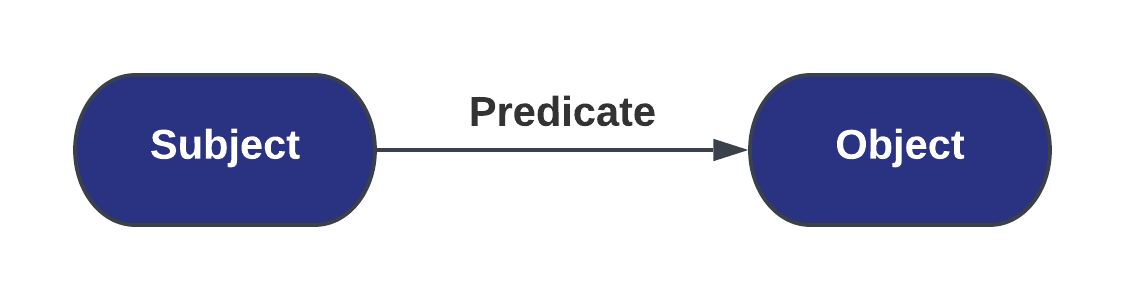
\includegraphics[scale=0.16]{graphics/rdf_triple_simple.png}
        \caption{Example of an RDF triple consisting of a subject, a predicate, and an object}
        \label{fig:rdf_triple_simple}
    \end{figure}
    
    Figure \ref{fig:rdf_graph_example} shows an RDF graph with two triples in its set. Both triple's subject is the URL of a web page. One triple also has the predicate \textbf{dc:title} and the object \textbf{Building}, whilst the other one has the predicate \textbf{dc:description} and the object \textbf{An ontology of a simple building}. As we can see, each of the RDF terms (subject-predicate-object) can be e.g. URLs or string literals.
    
    
    \begin{figure}[H]
        \centering
        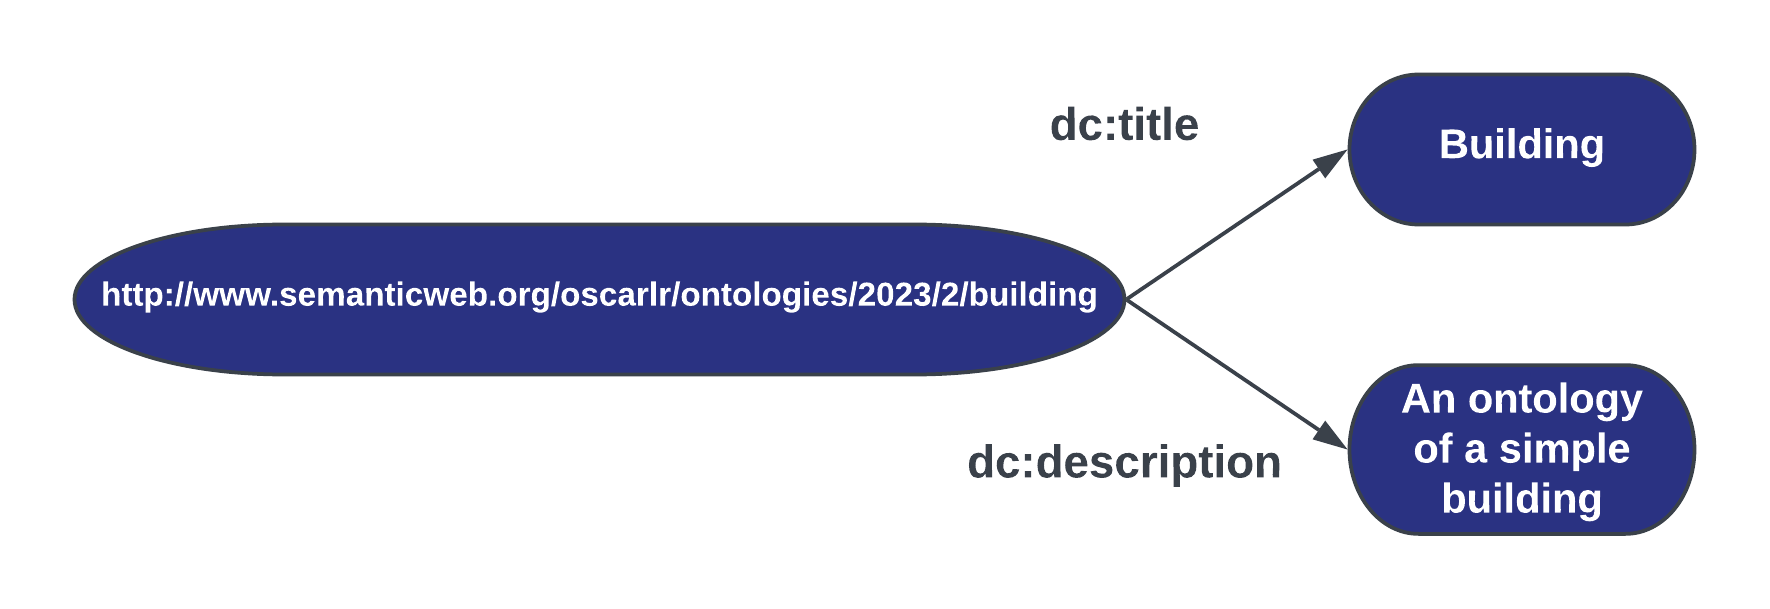
\includegraphics[scale=0.18]{graphics/rdf_graph_example.png}
        \caption{RDF graph consisting of two triples in its set}
        \label{fig:rdf_graph_example}
    \end{figure}
    \item \textbf{SPARQL}  is a query language for RDF and is defined by W3C. It expresses queries for varying sources of data, and the results from querying are sets of results or RDF graphs \cite{noauthor_sparql_nodate}.
    
    Below is an example of querying the title (\textbf{Building}) in the RDF graph shown in Figure \ref{fig:rdf_graph_example}.
\end{itemize}
\textbf{Data:}
\begin{Verbatim}[breaklines=true,breaksymbol=]
<http://www.semanticweb.org/oscarlr/ontologies/2023/2/building> 
<dc:title> 
”Building”
\end{Verbatim}
\textbf{Query:}
\begin{Verbatim}[breaklines=true,breaksymbol=]
SELECT ?title 
WHERE
{
  <http://www.semanticweb.org/oscarlr/ontologies/2023/2/building> 
  <dc:title> 
  ?title . 
}
\end{Verbatim}
\textbf{Result:}
\begin{table}[H]
    \begin{tabular}{|c|}
        \hline
        \textbf{title} \\
        \hline
        "Building" \\
        \hline
    \end{tabular}
    \caption{Query result}
    \label{tab:my_label}
\end{table}
    

\begin{itemize}
    \item \textbf{Web Ontology Language (OWL)} is a language for expressing rich knowledge of concepts (phrases in natural language) in an application domain \cite{szolovits_overview_1977}, as well as relations between entities. More specifically, ontologies describe domains in terms of classes, properties, and individuals \cite{bechhofer_owl_2009}.

    \item \textbf{Shapes Constraint Language (SHACL)} is a language for validating an RDF graph against a set of conditions as shapes expressed in another RDF graph. It is said that "data graphs" can be validated against "shapes graphs" \cite{noauthor_shapes_nodate}.
    
    \item \textbf{JSON-LD} JSON-LD is a JSON-based format for encoding and serializing linked data. Although not a well-established standard, it is still defined by W3C.  More specifically, it enables JSON objects to contain \emph{semantic} links \cite{noauthor_json-based_nodate}.
\end{itemize}

Commonly, these technologies can be used to create \emph{semantic} \hyperref[subsec:DigitalTwins]{digital twins}.

\subsection{Asset Model}\label{subsec:AssetModel}
Although BIM (Building Information Modeling) can be used with RDF and JSON to create static building infrastructure as mentioned in Section \ref{sec:Introduction}, some meaning is lost in translation due to a lack of semantic enrichment. BIM can be used in DTs for more context about the built environment which includes asset behavior \cite{godager_concept_2021}. However, a digital twin should aim to have interoperability between heterogeneous data sources.

OWL documents can easily be created (from export), loaded into, and maintained in ontology editors, such as Protégé\footnote{\url{https://protege.stanford.edu}}. Such a tool can be used to give semantics to e.g. a model of a building, as well as spending less time on creating and maintaining it compared to BIM. 

Figure \ref{fig:building_ontology} shows an example of an ontology of the simple building shown in Figure \ref{fig:simple_building} in Turtle Syntax (i.e. data format for RDF data model \cite{noauthor_terse_nodate}). This ontology uses semantic technologies outlined in Section \ref{subsubsec:Technologies}, such as RDF, which again is used by OWL to formalise knowledge in this specific building domain. For a more compact view of the ontology, URLs are removed and the coordinates of the room border corners are purposely left out, and some white space and comments are also removed. We also do not take directions into account meaning the room R1 will always be left of R2, and R2 always to the right of R1. Note that this is just an example of an ontology and that a real building domain would be many times more complex.

According to W3C's documentation, RDF graphs (such as the one shown in aforementioned Figure \ref{fig:building_ontology}) are static snapshots of information, but by giving appropriate vocabulary collections of Internationalized Resource Identifiers (IRIs) \cite{noauthor_rdf_nodate}, observations about entities or groups of entities through time can be captured.

Lastly, this ontology's data can also be reasoned over with technologies outlined in Section \ref{subsec:Reasoning}, which contains an example of reasoning over an \emph{inconsistent} ontology in Protégé (desktop version of editor), as well as a description on how to make the ontology \emph{consistent}.


\begin{figure}[H]
    \centering
    \caption{Ontology of a simple building with the object properties (hasDoor, hasWallLeft, hasWallRight), the classes (Room, Wall, Door), and the individuals (D, R1, R2, W)}
    \label{fig:building_ontology}
    \begin{Verbatim}[frame=single]
ex:hasDoor rdf:type owl:ObjectProperty .
ex:hasWallLeft rdf:type owl:ObjectProperty .
ex:hasWallRight rdf:type owl:ObjectProperty .

        
ex:Door rdf:type owl:Class .
ex:Room rdf:type owl:Class .
ex:Wall rdf:type owl:Class .

        
ex:D rdf:type owl:NamedIndividual ,
              :Door.
            
ex:R1 rdf:type owl:NamedIndividual ,
               :Room ;
      :hasWallRight :W .
    
ex:R2 rdf:type owl:NamedIndividual ,
               :Room ;
      :hasWallLeft :W .
    
ex:W rdf:type owl:NamedIndividual ,
              :Wall ;
     :hasDoor :D .
    \end{Verbatim}
\end{figure}

\subsection{SMOL}\label{subsec:SMOL}
SMOL is an imperative, object-oriented research language \cite{noauthor_smol_nodate-1}. According to the introduction of the SMOL language, it integrates semantic technologies, and can be used as a framework for creating DTs. For these DTs, the knowledge graphs can be used to capture asset models \cite{noauthor_introduction_nodate}.

The source code of SMOL is publicly available\footnote{\url{https://github.com/smolang/SemanticObjects}}. What follows is a simple SMOL program that creates a smartphone object and prints \verb|Careful!| if a criterion is met:

\begin{figure}[H]
    \centering
    \caption{A simple SMOL program}
    \label{fig:smol_program}
    \begin{Verbatim}[frame=single]
class Smartphone(Int id, String name, Boolean isBlackBerry) end

main
    Boolean isInsideRaspberryField = True;
    Smartphone blackberry = new Smartphone(1, "Evolve", True);

    if (blackberry.isBlackBerry & isInsideRaspberryField) then
        print("Careful!");
    end
end

    \end{Verbatim}
\end{figure}

\subsubsection{SMOL Interpreter}\label{subsubsec:SMOLInterpreter}
The interpreter reads and executes the SMOL program in a given file. The example program (in the file \textbf{example.smol}) shown in Figure \ref{fig:smol_program} was executed in the terminal. Note that the second and fourth line starts with \verb|MO>|. This simply means commands are executed inside the REPL.
\begin{Verbatim}[frame=single]
java -jar smol.jar
MO> reada example.smol
Careful!
MO>
\end{Verbatim}


\subsection{Reasoning}\label{subsec:Reasoning}
OWL was previously mentioned in Section \ref{subsubsec:Technologies} as a language for expressing rich knowledge of concepts and relations between entities. We should keep in mind, however, that this formalized knowledge should be reasoned over and put in context to draw conclusions based on criteria. There are many technologies that let us do this.
\subsubsection{HermiT}
HermiT is a reasoner for OWL 2 \cite{glimm_hermit_2014}, which is an upgraded version of OWL. \citeauthor{glimm_hermit_2014} describes that the reasoner support both object and data property classification, as well as SPARQL query answering. HermiT is built into the ontology editor Protégé and can be used to reason over an ontology directly in the editor. Other plugins for reasoning can be added to the ontology editor, but it is convenient that HermiT comes with the installation.

Figure \ref{fig:hermit_in_protege} shows an ontology that is \emph{inconsistent} (an ontology that cannot have any models and entails everything \cite{horridge_explaining_2009, huang_reasoning_2004}). The information window \textbf{Help for inconsistent ontologies} tells us that the OWL reasoner (HermiT) will no longer be able to provide any useful information about the ontology. The ontology is inconsistent because the object properties \textbf{hasWallLeft} and \textbf{hasWallRight} are disjoint (having no elements in common), and the individual \textbf{R1} has both object properties. This makes no sense because the room can't have the wall on its left side and at the same time have it on its right side. This could be fixed by simply removing the object property \textbf{hasWallLeft} from the individual according to the context. The effect of an inconsistent ontology is that no meaningful conclusions can be drawn from it \cite{horridge_explaining_2009}.

\begin{figure}[H]
    \centering
    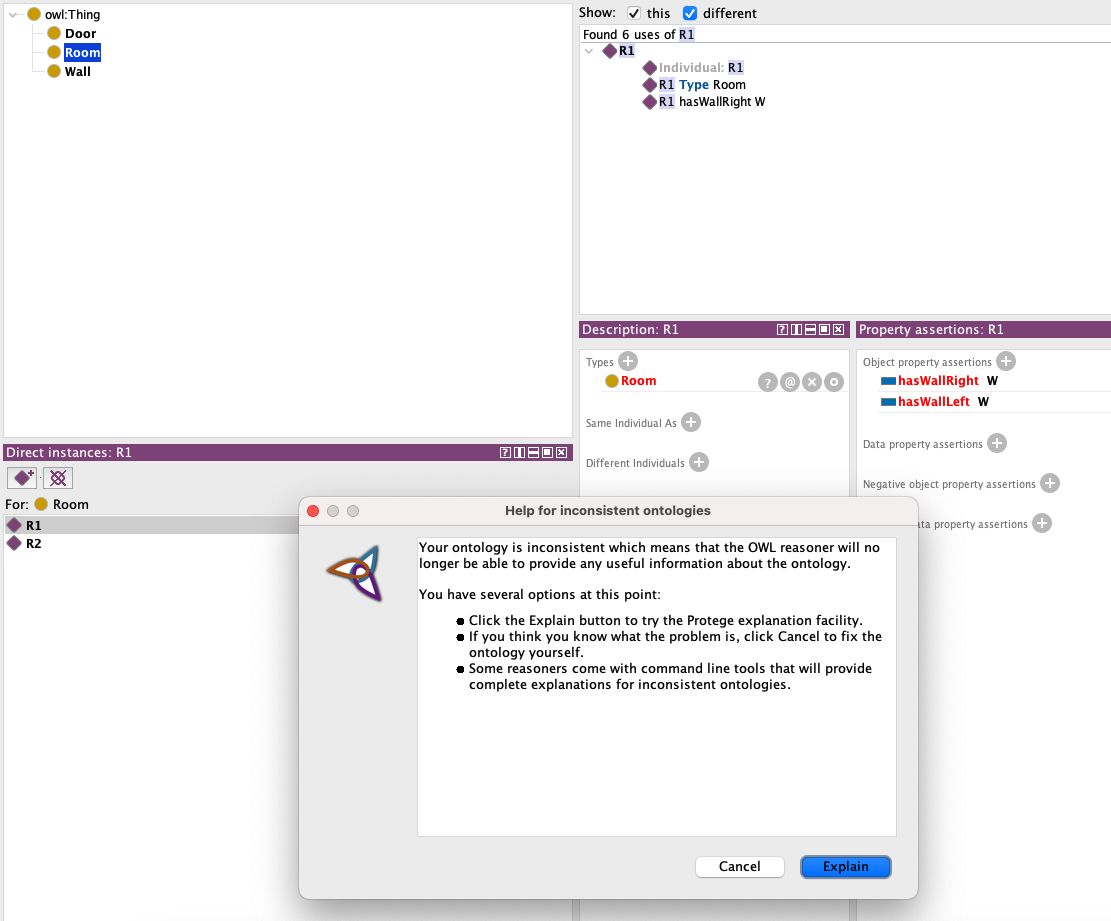
\includegraphics[scale=0.30]{graphics/screenshot_ontology.png}
    \caption{Shows use of HermiT to reason over an ontology in Protégé}
    \label{fig:hermit_in_protege}
\end{figure}

There also exist other technologies that provide reasoner tools. Some notable mentions include, but are not limited to:
\begin{itemize}
    \item{\textbf{Apache Jena}} is an open source framework that has the Inference API which include reasoner tools that can be used to reason over data, as well as checking content of triple stores \cite{noauthor_apache_nodate-1}. The source code is publicly available\footnote{\url{https://github.com/apache/jena}}.
    \item{\textbf{OWL API}} is a Java framework that lets us create, serialize or manipulate ontologies written in OWL \cite{noauthor_owl_nodate}, and its source code is openly accessible\footnote{\url{https://github.com/owlcs/owlapi}}. Its recent development is more focused towards OWL 2 however.
    \item\hyperref[subsec:SMOL]{\textbf{SMOL}} provide reasoning tools through its interpreter, which implements \emph{semantic lifting} (i.e. generating a knowledge graph from the current state of a SMOL program) \cite{noauthor_semantic_nodate}. 
    
    The knowledge graph is generated by using the \verb|dump| command in SMOLs Read-Eval-Print Loop (REPL) (i.e. user inputs in a terminal are read and results are returned to the user). The knowledge graph is generated as an output file with the filename extension \verb|.ttl|. Reasoning is done automatically by the interpreter whenever \verb|access| or \verb|member| are executed. Apache Jena reasoner is used for \verb|access|, whilst \verb|member| triggers reasoning over an OWL concept with HermiT. Validating with SHAQL does however not require reasoning.
\end{itemize}



\subsection{App Development}\label{subsec:AppDevelopment}
We will describe the topic of app development by looking at concerns when developing in industry. Smartphones and tablets have different operating systems for mobile, in which the two most notable are iOS (iPhone and iPad) and Android (smartphones and tablets with different brands, such as Samsung, Google, and OnePlus). Smartphones are heterogeneous by nature. They not only have different operating systems but also have various device sensors, depending on the brand and price of the device. 

One should develop for multiple platforms from a single codebase, provided that development time is crucial and that the app should have cross-platform (e.g. both iOS and Android) support. However, this should be planned early on in the development, preferably before anyone starts writing code. Some examples of frameworks that support cross-platform app development include:

\begin{itemize}
    \item Flutter
    \item Ionic
    \item React Native
\end{itemize}

Devices are often equipped with a GPS (Global Positioning System), which gets signals from satellites to determine the GPS-based physical location of the device. Google provides a service, namely Google Location Accuracy, which collects additional location data from multiple sources, such as nearby Wi-Fi and cellular networks, to provide a more accurate physical location of a device \cite{noauthor_how_nodate}. The Google Maps SDK is a set of tools for integrating maps into applications, such as for Android and iOS. According to Google, some features of the Software Development Kit (SDK) are different map displays and map gesture responses \cite{noauthor_maps_nodate}. 

Continuous tracking of physical devices raises privacy concerns. General Data Protection Regulation (GDPR)\footnote{\url{https://gdpr-info.eu/}} works to ensure the privacy and security of personal data. As an example, no personal data should be collected without the permission of the \emph{data subject} (i.e. user), stated in GDPR Article 13 and 14 \cite{noauthor_guide_nodate}, and for what purpose the data is collected should be explicitly stated.

\subsection{Databases}\label{subsec:Databases}
Databases are collections of information that exist for a long time, often over many years \cite{garcia-molina_database_2002}. They can be divided into relational and non-relational (NoSQL) databases \cite{mohamed_relational_2014}. Relational databases have existed for many decades and store data in tables (which consist of columns and rows), whilst \emph{NoSQL} (i.e. not only SQL) databases store data differently. Examples of relational databases are MySQL and PostgreSQL, whereas examples of NoSQL databases are: 
\begin{itemize}
    \item \textbf{MongoDB} is a well-known NoSQL database for storing data in JSON documents and its source code is publicly available\footnote{\url{https://github.com/mongodb/mongo}}.
    \item \textbf{Firebase Realtime Database} is a cloud-hosted NoSQL database that stores data as JSON objects  \cite{noauthor_firebase_nodate}. Furthermore, data is synchronized in real-time to cross-platform clients.
    \item \textbf{InfluxDB} is a NoSQL database for storing \emph{time series data} (i.e. "sequence of data points indexed in time order" \cite{noauthor_what_nodate})  \cite{noauthor_influxdb_nodate}, and its source code is also openly accessible\footnote{\url{https://github.com/influxdata/influxdb}}. Flux queries can be used to query time series data in the database.
\end{itemize}

According to \citeauthor{garcia-molina_database_2002}, databases are managed by a Database Management System (DBMS), a system that should:
\begin{itemize}
    \item Let users create new databases in which the logical structure of data (schema) is specified by the user using a data-definition language.
    \item Let users query and modify data with a query language.
\end{itemize}

Non-relational variants have become increasingly popular in recent years due to how they solve scalability concerns with relational databases. NoSQL databases are of different types, such as document databases and graph databases. As described by \citeauthor{mohamed_relational_2014}, traditional databases were not created with horizontal scaling (sharding) in mind. More specifically, it does not do well with new machines being added to the pool of resources. Instead, it relies heavily on vertical scaling, which is adding more computing power (CPU, RAM) to an individual resource (machine) in the pool. On the other hand, NoSQL databases are optimized for scaling horizontally \cite{mohamed_relational_2014, kim_geoycsb_2023}.

We should consider that although databases can have many different uses, some are better for specific purposes than others. Time series databases can be integrated into digital twins (DTs) for getting updated sensor data from the physical twin (PTs). Section \ref{subsec:SMOL} describes that SMOL can be used as a framework to create DTs. Additionally, in SMOL we can query time series data from InfluxDB by using the \verb|access| statement \cite{noauthor_time_nodate}. An example program of querying latitude and longitude coordinates from the start of the time range, and then returning the list of coordinates follows:

\begin{figure}[H]
    \centering
    \begin{Verbatim}[frame=single,breaklines=true]
List<Double> getCoordinates()
    List<Double> coordinates = null;
    coordinates = access(
        "from(bucket: \"Data\")
        |> range(start: 0)
        |> filter(fn: (r) => r[\"_measurement\"] == \"data\")
        |> filter(fn: (r) => r[\"_field\"] == \"latitude\" or r[\"_field\"] == \"longitude\")
        |> aggregateWindow(every: 5m, fn: mean, createEmpty: false)
        |> yield(name: \"mean\")",
        INFLUXDB("influx.yml")
    );
    return coordinates;
end
    \end{Verbatim}
    \caption{Accessing time-series data from InfluxDB in a function written in SMOL}
    \label{fig:access_time_series}
\end{figure}
    

Firebase Realtime Database has multi-platform support for clients, such as support for Android and iOS devices \cite{noauthor_firebase_nodate}.



\newpage
\section{Problem analysis and design}\label{sec:Analysis}
Given the gap that was identified in Section \ref{subsec:Motivation}, the hypothesis (H) and its three guiding research questions (RQ1, RQ2, RQ3) described in Section \ref{subsec:ProblemStatement} will in this chapter be examined based on the theoretical background information and general code examples in Section \ref{sec:Background}. We create a building domain based on the analysis of the research questions. Then we examine what a dynamic asset model entails, and how static data can be separated from dynamic data in it. Different technologies, such as databases, frameworks for creating applications (apps), and semantic digital twins are considered. Lastly, we present the resulting structural requirements as the basis for the implementation.

\subsection{Research questions (RQ1, RQ2, RQ3)}
\subsubsection{RQ1}\label{subsubsec:RQ1}
RQ1 is concerned with creating a dynamic asset model of a simple building. From the descriptions of asset models in Section \ref{subsec:AssetModel}, an ontology of a simple building was created, as shown in Figure \ref{fig:building_ontology}. This asset model is a simplified version of an exported OWL document (file). It can be created in an ontology editor, such as Protégé. Although other ontology editors can be used, we should use Protégé due to its user-friendliness and the extensive documentation provided in its user guide \cite{horridge_practical_2011}. This exported file is provided to and used by the digital twin (DT) by using the SMOL interpreter.

RQ1 is also concerned with creating an asset model that is \emph{extensible}. Being extensible in this context means that an operator should be able to manually add new smartphones that have no registered physical location, or add existing building infrastructure to the ontology. We provide a template for movable entities, which is used to add new movable entities to the domain according to context. More specifically, new smartphone individuals without physical location data are added to the asset model. The usage of the template is shown below. Changeable parts in the template are highlighted. This should be added to the OWL document (file), either by the server or manually by an operator:

\begin{Verbatim}[commandchars=\\\{\}, breakanywhere=true]
### \hl{http://www.semanticweb.org/oscarlr/ontologies/2023/2/building#smartphone5}
\hl{:smartphone5} rdf:type owl:NamedIndividual ,
                      :MovableEntity ;
             :movableEntityId "\hl{5}" .
\end{Verbatim}  

Section \ref{subsubsec:DynamicAssetModel} further examines what a \emph{dynamic} asset model entails.

\subsubsection{RQ2}\label{subsubsec:RQ2}
RQ2 asks whether we can "enable bidirectional data flow between the PT and DT, such that the digital twin gets updated sensor data from the mobile devices in the PT and sends informed decisions back". Bidirectional data flow is data that is exchanged both ways, and not just in one direction between the physical twin (PT) and digital twin (DT), or vice versa. The DT observes the PT in near real-time and gets updated sensor data from its physical counterpart. The DT should then send informed decisions back to it. A lot of value is derived from the DT making an informed decision on behalf of a mobile asset in the PT, and it is crucial that the appropriate smartphone user is notified.

The DT could conclude to make an informed decision if some criteria are met. Although quite obvious, we will exemplify this by checking if a point is inside an area. Using what is shown in Figure \ref{fig:simple_building} as a basis, an area's two border corners are expressed as follows:
\begin{enumerate}
    \item $(x_1, y_1)$
    \item $(x_2, y_2)$
\end{enumerate}
Meaning, to check if a smartphone's physical location (point) $(x, y)$ is inside the area, we can check if the following is true:\newline\newline$(x >= x_1\:\land\: x <= x_2)\:\lor\:(x >= x_2\:\land\:x <= x_1)$\newline$\land$\newline$(y >= y_1\:\land\:y <= y_2)\:\lor\:(y >= y_2\:\land\:y <= y_1)$\newline\newline Note that we include both directions so maintainers can freely choose border corners for an area, which gives flexibility to the extensible asset model and aligns with RQ1 described in Section \ref{subsubsec:RQ1} above.

\subsubsection{RQ3}
RQ3 is concerned with how we can "separate dynamic data (smartphone’s physical location) from static data
(building infrastructure) in the asset model". Hypothesis (H) states that the asset model should be of a simple building. The rooms with a square area constitute it. In contrast to building infrastructure, mobile assets that are tracked can change at any time, as well as their continuously changing physical locations. As described in Section \ref{subsec:Scope}, we are not concerned with other movable entities in the building domain apart from the mobile assets. And, even though the data of the building infrastructure may change, it will not change during program execution in SMOL. This is not the case with the time series data accessed from InfluxDB in SMOL. However, one way to separate the dynamic data from the static data is by examining \emph{how} often changes occur through time, where separate means not affecting one another. More specifically, when reloading the asset model, the static data should not be affected by the data data considered dynamic. Further analysis of static and dynamic data is described in Section \ref{subsubsec:StaticAndDynamicData}, and also later discussed in Section \ref{subsec:DiscussDynamicData}.


\subsection{Building domain}\label{subsec:BuildingDomain}
From considering the three research questions, we have created a possible domain including a built environment based on static data, as well as movable entities with their physical location as dynamic data, as shown in Figure \ref{fig:static_built_environment}. \textbf{Physical 2D space} is provided for the context of outside and is in two dimensions as described in Section \ref{subsec:Scope}. This means that altitude is not taken into account. Note that the relationships between some entities use \emph{composition} (i.e. indicates a very strong relationship between the entities, which means that if the owing entity (e.g. \textbf{Physical 2D space}) is destroyed, so is the entity linked to it (e.g. \textbf{Building} \cite{pilone_uml_2005}) (it can be thought of as a black hole..)

\begin{figure}[H]
    \centering
    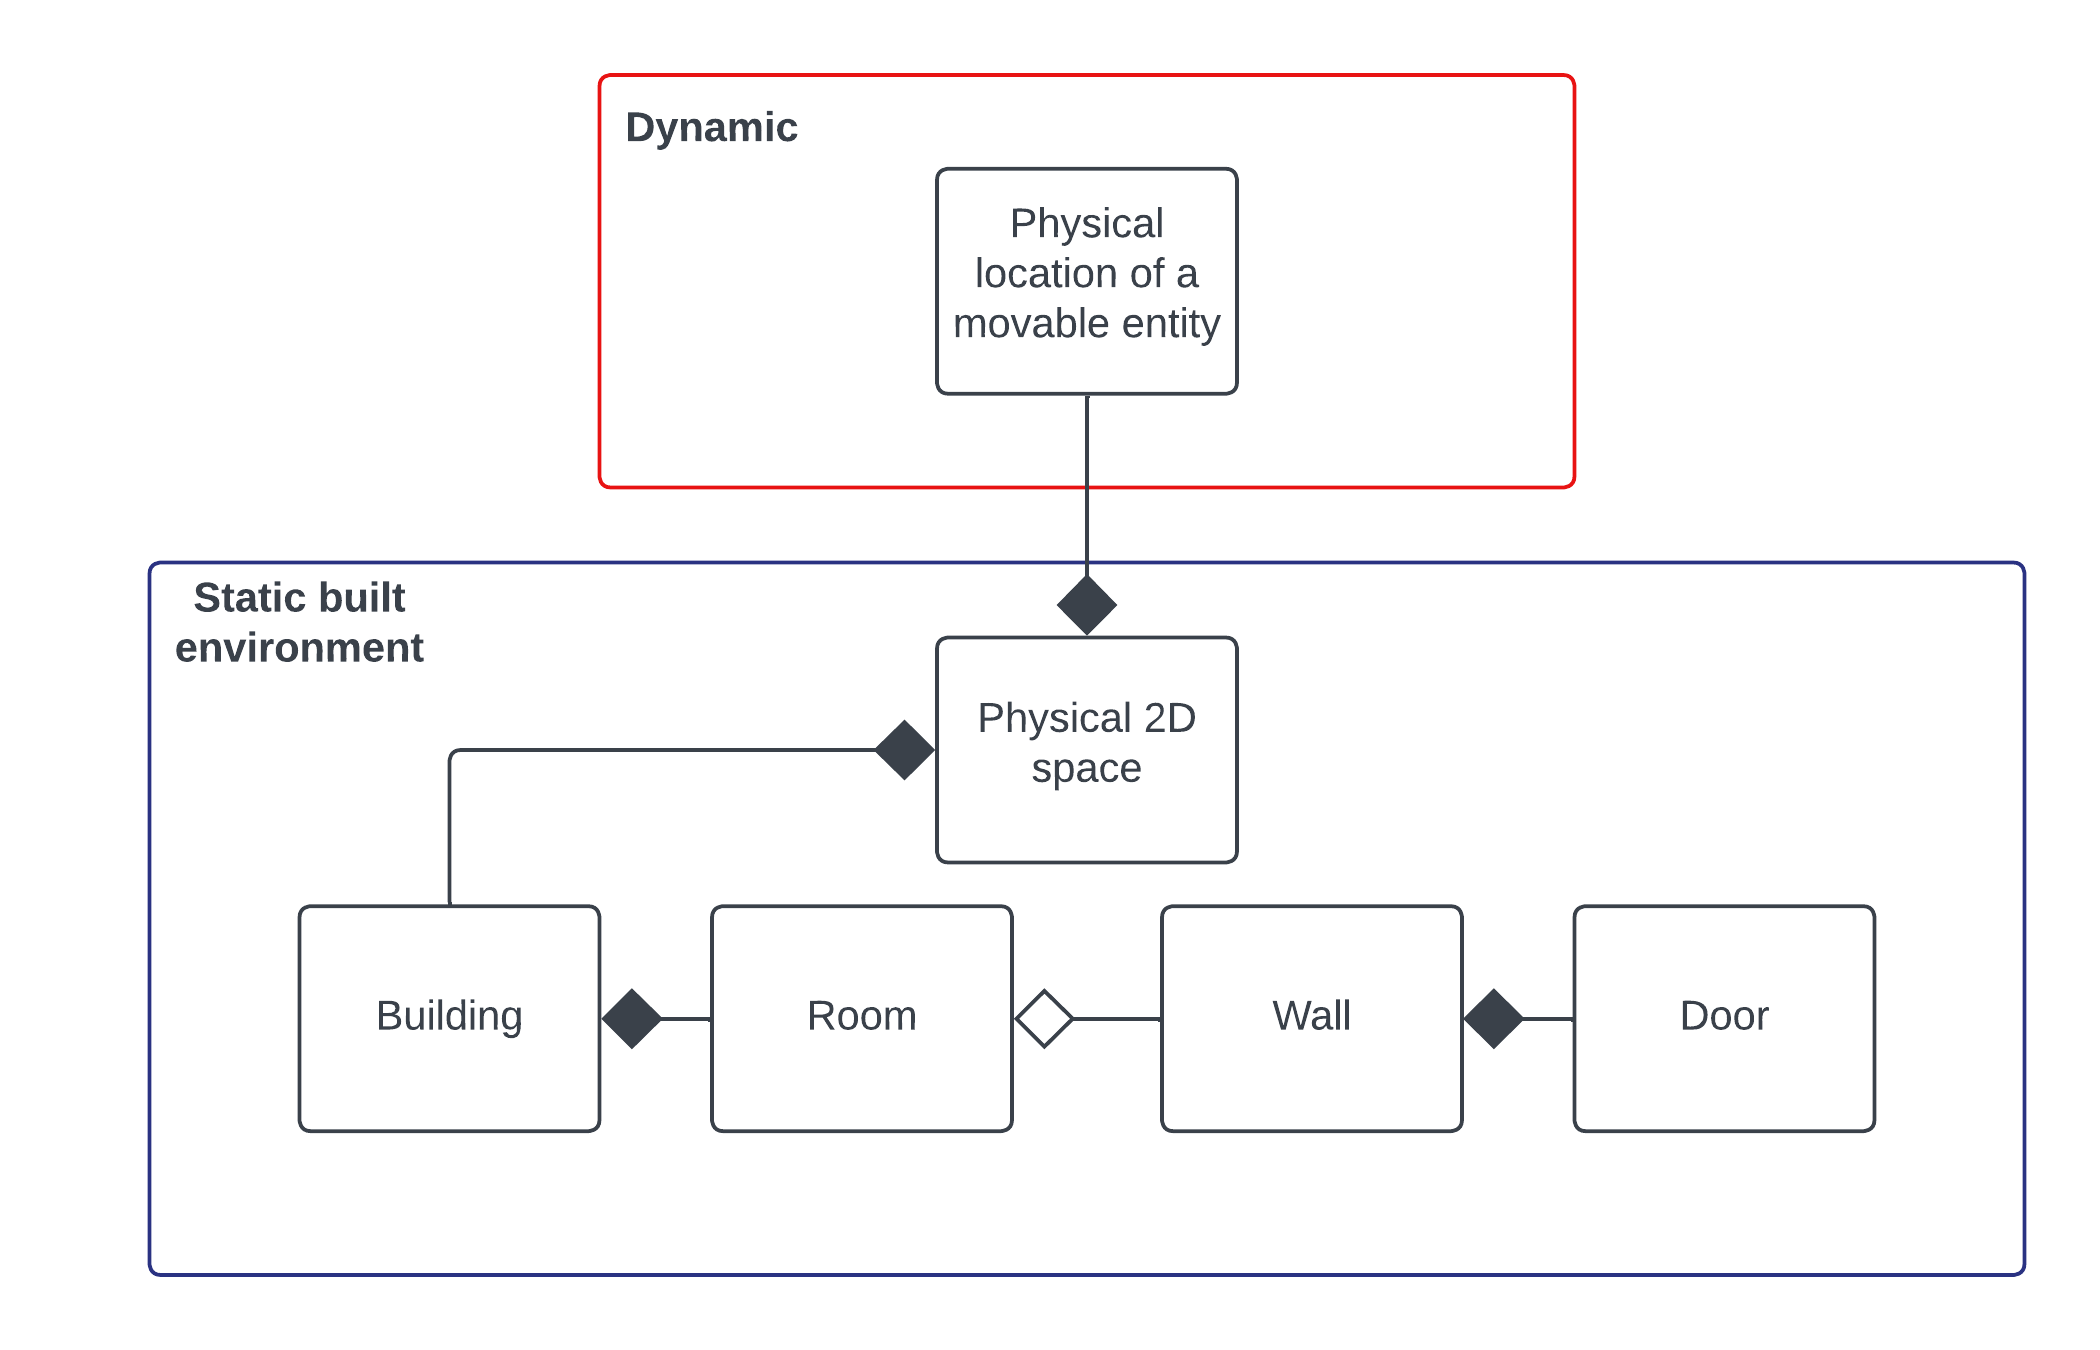
\includegraphics[scale=0.16]{graphics/static_built_environment.png}
    \caption{A UML class diagram that illustrates the separation of static and dynamic behavior}
    \label{fig:static_built_environment}
\end{figure}


\subsection{Dynamic asset model}\label{subsubsec:DynamicAssetModel}
Section \ref{subsec:AssetModel} describes concerns with BIM (Building Information Modeling), and how ontologies (asset models) created with semantic technologies deal with these concerns. Another concern with BIM worth mentioning is that it does not handle dynamic behavior very well \cite{kamburjan_digital_2022}.

Simply put, a \emph{dynamic} asset model is an ontology in which some data changes through time. If we were to export the ontology created in Protégé, we would get an OWL document (file) that would describe the domain in terms of classes, properties, and individuals. Changing the ontology in any way (e.g. adding another movable entity) would represent a new RDF (Resource Description Framework) graph.

Figure \ref{fig:building_ontology} shows an exported ontology of a building in Turtle Syntax. The ontology editor lets us specify the format of the ontology to be exported. From creating this ontology as a basis for our future ontology implementation, we discovered that it would be necessary to create a common class for \emph{atleast} the movable entities (individuals) due to the sheer number of them in the GUI (Graphical User Interface) in Protégé, as well as to formalize the knowledge of heterogeneous smartphones.

A digital twin (DT) based on a \emph{dynamic} asset model should be able to recognize the following, according to the generated knowledge graph:
\begin{itemize}
    \item Manual changes of static data by an operator
    \item Automatic updates of dynamic physical location data from the server
\end{itemize}
\subsection{Data separation}
In this section, we are further analyzing the separation of static and dynamic data and giving some practical examples to support this. First, we describe and illustrate how they can be separated in the asset model and in SMOL. Then we examine how we can separate the static analysis of what a critical area \emph{is} from the dynamic snapshots of smartphones at a certain point in time.

\subsubsection{Static and dynamic data}\label{subsubsec:StaticAndDynamicData}
Figure \ref{fig:static_dynamic_asset_model} shows the separation of static and dynamic data. The \textbf{Asset Model} \emph{don't} have dynamic physical location data, but the smartphone individuals and their IDs as static data instead. The SMOL program accesses the smartphones by their IDs with \verb|access|, and adds the dynamic data from InfluxDB according to the IDs. \textbf{Place} consists of area(s) with predefined border corner coordinates and is static data. We take notice that a server could continuously update the time series database with the physical locations of the mobile devices, as well as add the smartphone individuals to the asset model.

\begin{figure}[H]
    \centering
    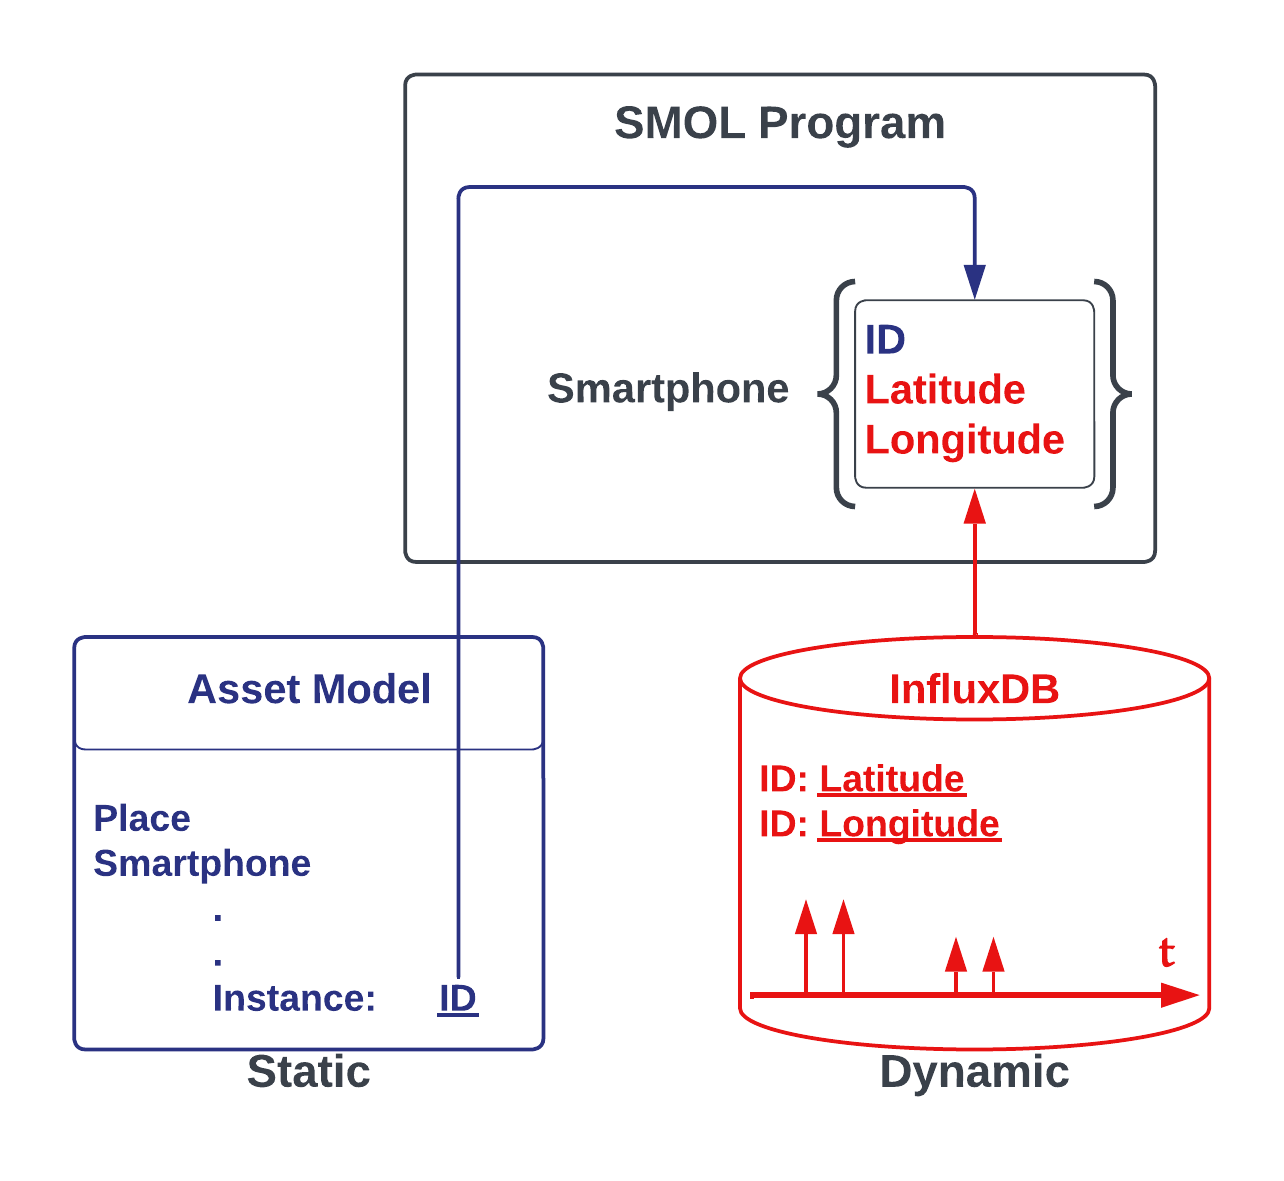
\includegraphics[scale=0.22]{graphics/static_dynamic_asset_model.png}
    \caption{The separation of \textbf{Static} and \textbf{Dynamic} data, illustrated in blue and red, respectively}
    \label{fig:static_dynamic_asset_model}
\end{figure}

The aforementioned figure also shows the direction of data flow between the \textbf{Asset Model} and \textbf{SMOL}, and \textbf{InfluxDB} and \textbf{SMOL}. The SMOL program accesses the static data (\textbf{Place} and instances of \textbf{Smartphone}) in the asset model and gets the updated sensor data of the smartphones from InfluxDB. The SMOL program then creates \textbf{Smartphone} objects from the data.


\subsubsection{Further data separation}\label{subsubsec:FurtherDataSeparation}
If we were to illustrate querying an asset model with a SPARQL query (SPARQL Query Language for RDF), the consensus is to use red color for core parts of SPARQL syntax or language, whilst the color blue is used for examples of query-specific values or text that goes into SPARQL queries \cite{noauthor_sparql_nodate}. Keeping this in mind, we still use blue text color for static data and red text color for dynamic data in this thesis because they are, respectively, calming or disruptive. 

It is important to look at the differences between the sensor data and the informed decisions in terms of what the data can be used for. The DT gets updated sensor data from the PT, and sends informed decisions back, as RQ2 states. The updated sensor data from the PT is the newest physical location from the mobile assets in the PT. It is crucial that the PT can use this data \emph{as is}, and therefore the data should be exact coordinates (latitude, longitude), and identifiable. We should think about what an informed decision means. An informed decision is a conclusion made by the DT when there is sufficient information to determine something on behalf of the PT to control it. An example of this is the DT sending warnings back to the PT when the DT has determined that smartphones are inside critical areas. The analysis of what a critical area \emph{is} however, is not taken into account, as stated in Section \ref{subsec:Scope}. Therefore, the DT should not decide that an area is dangerous. This could be a job for an operator responsible for defining the areas in the asset model. 

Lastly, we should separate the static analysis of what a critical area is from the dynamic snapshots of smartphones at a certain point in time. This way the dynamic behavior doesn't affect the static behavior. Some background information on a digital shadow (DS) was given in Section \ref{subsec:DigitalTwins}. A DS could be created to handle one-way data flow and to further separate data, as well as give modularity to our implementation.

\subsection{Analysis of technologies}
In this section, we analyze different technologies from the descriptions of them in Chapter \ref{sec:Background}. These technologies can be used to realize the proposed high-level architecture in Figure \ref{fig:initial_components}. Choices of architectural components are justified based on the analysis of the problem space. We look at time series databases and real-time databases, frameworks for creating cross-platform apps, and semantic digital twins.

\subsubsection{App Development}\label{subsubsection:AppDevelopment}
From the background information on app development provided in Section \ref{subsec:AppDevelopment}, we chose to focus on Flutter as a framework for creating cross-platform applications (apps) due to a number of reasons. We considered other frameworks for creating apps for iOS and Android from a single codebase as well, such as Ionic and React Native. However, we had no prior experience with either, and Flutter has great documentation provided by Google, and is popular in the industry. It was also made clear in the background section on App Development that Google Maps SDK should be used to integrate Google Maps into the Flutter app.

The programming languages were seen as tools that came with the choice of frameworks and were thus not focused on that much. However, the programming language used in Flutter applications is Dart, which is also developed by Google. React Native and Ionic apps are both written in JavaScript. Ionic apps can be written using a single code base in the libraries React, Angular, or Vue \cite{noauthor_ionic_nodate}.

\subsubsection{Databases}\label{subsubsection:Databases}
There exist many databases, but Section \ref{subsec:Databases} narrowed the choices down to the time series database InfluxDB and the real-time database provided by Firebase. 

SMOL, as a framework for creating digital twins (DTs), supports InfluxDB and provides open-source examples for querying time series data which made it an easy choice. 

When it comes to real-time databases, we saw that the real-time database by Firebase is based on web-sockets, which is more performant than polling due to data being accessed in real-time and due to low latency. There is also no limit to the number of nodes that can be pushed to a list in Firebase, which let us handle an unlimited number of smartphones as stated in Section \ref{subsec:Scope}. Although this can be very costly if the user base scales out of proportion. Redis was also considered as a real-time database that could be used for our implementation, but we had prior experience with Firebase, and integrating it should take less time. It is a cloud-hosted solution \cite{noauthor_firebase_nodate}, but one can download the Google Cloud SDK Shell to authenticate and interact with the services provided by Firebase.

Furthermore, using a database in the communication between clients and the server allows for an operator to easily check the assigned clients, as well as which clients should be informed. From the prototypical implementation, it was made clear that \emph{real physical devices} (not just emulated ones) should be detected by the physical twin (PT). 

Lastly, we should ask ourselves why we should use a real-time database in our client-server communication, but this is later discussed in Section \ref{subsec:ClientServerCommunication} where we also look at FastAPI and the communication between architectural components.

The \textbf{Server} in Figure \ref{fig:initial_components} has not been explicitly described yet in this thesis as its main function was to enable a bidirectional flow of data between the PT and the digital twin (DT). Most people in general are familiar with Java,  a well-known and established programming language, and our fellow students are quite familiar with its syntax as well. Lastly, The OWL API and Apache Jena have many open-source examples in Java, which is another reason we should use Java in our server implementation and not e.g. Kotlin (which the SMOL interpreter is written in). 

\subsubsection{Semantic Digital Twin}\label{subsubsec:SemanticDigitalTwins}
Section \ref{subsec:SMOL} describes that SMOL (Semantic Micro Object Language) can be used as a framework for creating digital twins (DTs) and that it integrates semantic technologies. Knowledge graphs can be generated by using the \verb|dump|-command in the REPL provided by the SMOL interpreter. The knowledge graph can capture a knowledge base, such as a dynamic asset model, in which static data is separated from dynamic data. This asset model combined with the SMOL program, produces the knowledge graph. It is also possible to access the asset model from the SMOL program. As SMOL also integrates semantic languages, such as SHACL for validation and SPARQL for querying, it could be a good fit for our implementation.

\subsection{Structural requirements}\label{subsec:Requirements}
We have analyzed the research questions, the building domain, and the dynamic asset model in which static and dynamic data are separated. Technologies have also been examined and justified. From this, we create the structural requirements for the implementation, which is an \emph{unordered} nested list in which all levels are also \emph{unordered}. It is structured into the parts \textbf{Client}, \textbf{Server}, \textbf{Databases}, and \textbf{Digital Twin}.
\newline

\noindent\textbf{Structural requirements:}
\begin{itemize}
    \item \textbf{Client}
    \begin{itemize}
        \item Can choose to send its newest status (ID, latitude, longitude) 
        \item Appropriate endangered clients are warned 
        \item Show appropriate in-app messages to the user
        \item Ask for permission to track the physical loation of the device
        \item Clearly show when the physical location of the device is tracked
        \item Clearly show when the physical location of the device is \emph{not} tracked
    \end{itemize}
    \item \textbf{Server}
    \begin{itemize}
        \item \textbf{1.} Forward the sensor data to a time series database
        \item \textbf{2.} Forward the informed decisions to a real-time database
        \item Should be possible to do \textbf{1.} and \textbf{2.} above at the same time
        \item Reload asset model with tracked clients
        \item Access and read the generated knowledge graph
    \end{itemize}
    \item \textbf{Databases}
    \begin{itemize}
        \item Realtime database
        \begin{itemize}
            \item Store the ID and physical location of the clients
            \item Store data about which clients the DT made an informed decision for
        \end{itemize}
        \item Time series database
        \begin{itemize}
            \item Store the time series data
        \end{itemize}
    \end{itemize}
    \item \textbf{Semantic Digital Twin}
    \begin{itemize} 
        \item \textbf{3.} DS gets the newest sensor data from the time series database
        \item \textbf{4.} Access the smartphones in the asset model by their IDs
        \item Create smartphone objects by combining data from \textbf{3.} and \textbf{4.} above 
        \item Access the critical areas from the asset model
        \item Check if smartphones are inside any critical areas
        \item Handle new smartphones that don’t have a physical location
        \item Provide examples of SPARQL queries
        \item Show informative messages in the REPL during program execution
    \end{itemize}
\end{itemize}

In addition to this, operators should be able to access the knowledge graph and edit the asset model either offline or online. Lastly, it should be possible for an administrator to check the data stored in both the real-time database and the time-series database, whilst protecting clients' privacy as much as possible.

\subsection{Design}\label{subsec:Design}
Having the structural requirements described in Section \ref{subsec:Requirements} for the \emph{client} in mind, in addition to the analysis of app development, and the background information on GPS sensors in Section \ref{subsec:AppDevelopment}, a wireframe was created. We justify creating this without any input from conducting user studies because it can be seen as a standard map screen in an app, due to similarities with the official Google Maps app. We should however create our own version of the location button, referencing the requirements of the client. Figure \ref{fig:wireframe_app} shows the wireframe of the User interface (UI) of the map screen in the app. Simply put, the UI is what the user \emph{sees} in the app, and is built from the widgets in Flutter, behaving much like components in e.g. React.

\begin{figure}[H]
    \centering
    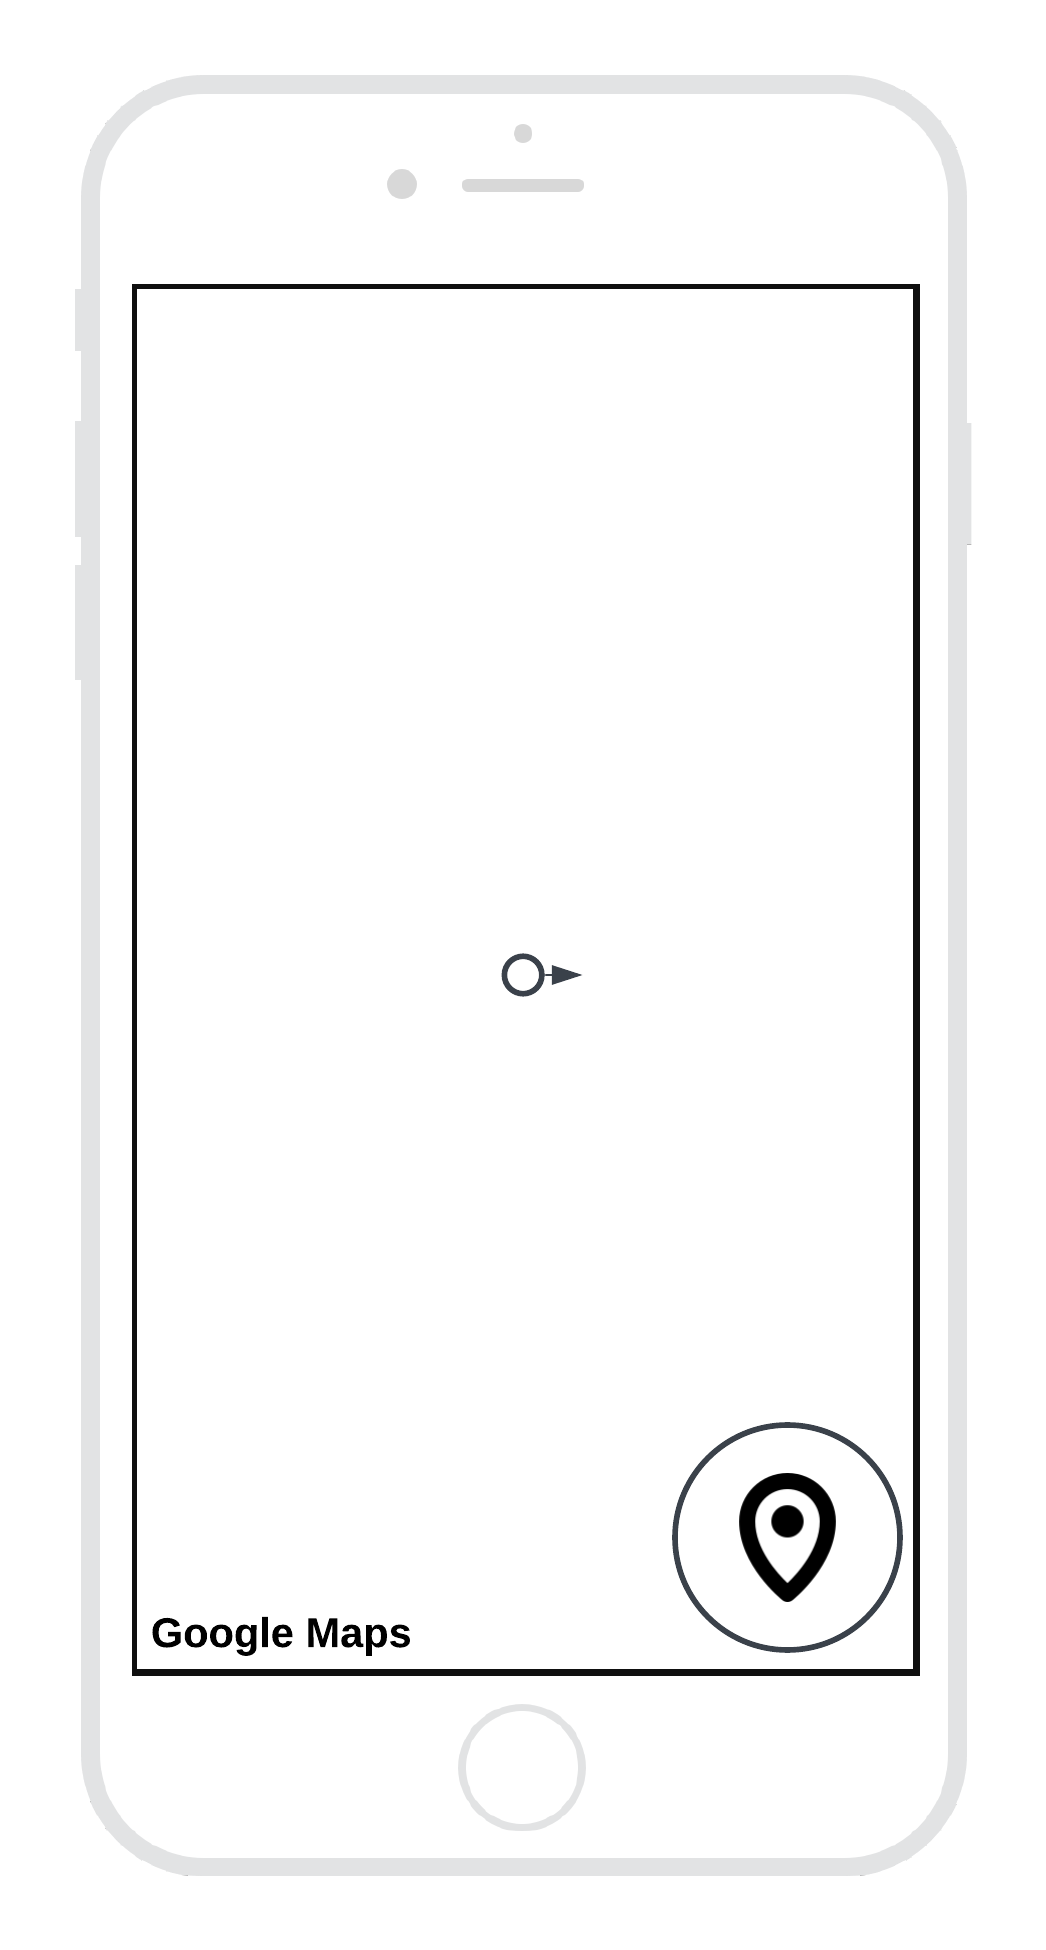
\includegraphics[scale=0.12]{graphics/wireframe_app.png}
    \caption{Shows a wireframe of the UI in the app}
    \label{fig:wireframe_app}
\end{figure}


\newpage
\section{Implementation}\label{sec:Implementation}
This chapter describes the proof-of-concept implementation, which is publicly available\footnote{\url{https://github.com/Owlar/Master-Thesis}}, based on the structural requirements in Section \ref{subsec:Requirements}, by describing each of the following parts in it:
\begin{itemize}
    \item Client
    \item Server
    \item Databases
    \item Semantic Digital Twin
\end{itemize}
In the first section, we describe the implementation of a prototype based on the initial architectural components in Figure \ref{fig:initial_components}. 

Then we look at the final version in Figure \ref{fig:components}, and describe what was implemented. For each of the larger architectural components in the figure, we reference the section that describes it in Chapter \ref{sec:Background}, and the design decision that enables it in Chapter \ref{sec:Analysis}. We also reference the corresponding \emph{item} in the structural requirement \emph{part} we are in.

\begin{figure}[H]
    \centering
    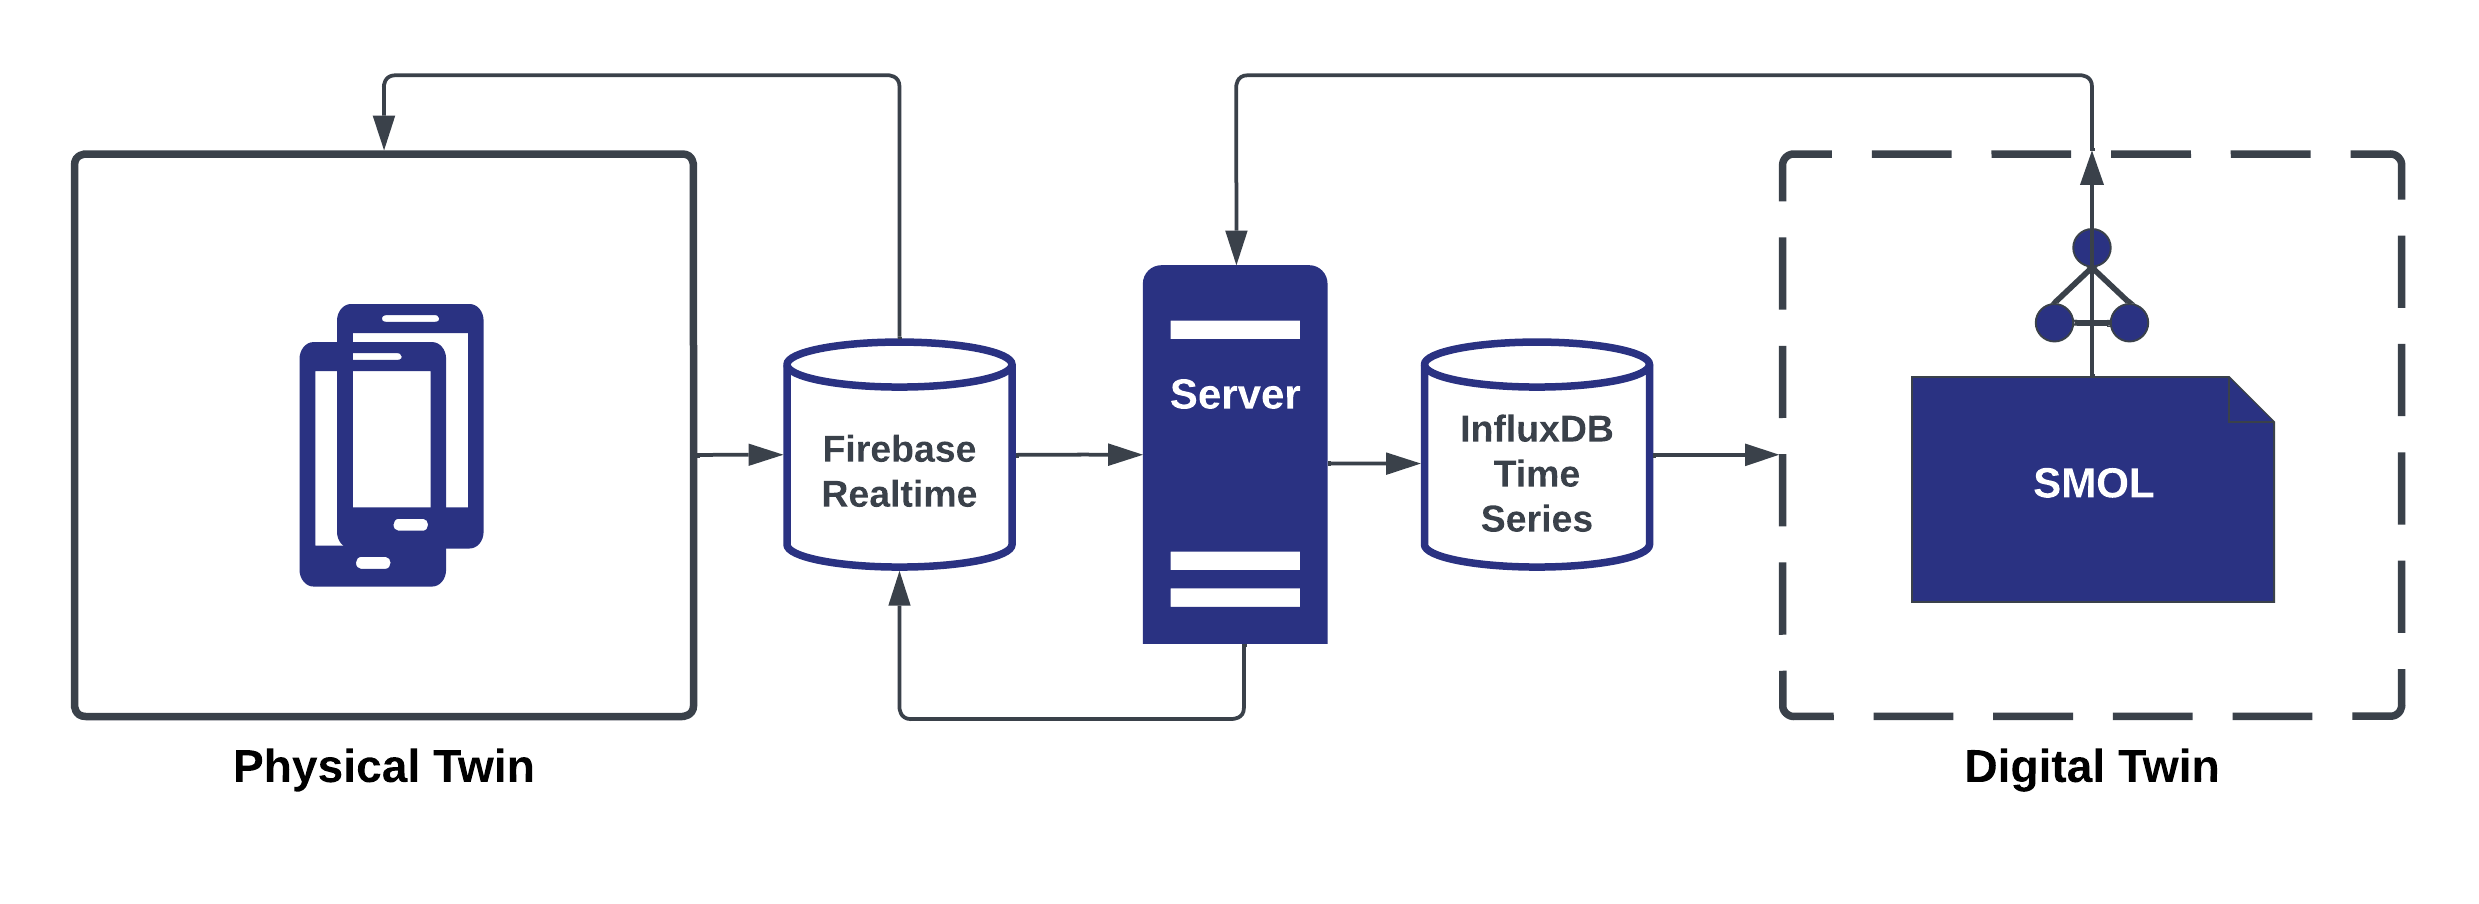
\includegraphics[scale=0.14]{graphics/thesis_overview.png}
    \caption{Overview of architectural components of the final implementation in this thesis}
    \label{fig:components}
\end{figure}

\subsection{Prototypical implementation}\label{subsec:Prototypical}
Due to the extensive architecture, we early chose to implement an app prototype by letting all of the architectural components in Figure \ref{fig:initial_components} communicate first. The \textbf{Physical Twin} in the figure consists of \textbf{Mobile Assets} which are smartphones. Based on the background information in Section \ref{subsec:AppDevelopment}, and from further narrowing of the technologies in Section \ref{subsubsection:AppDevelopment}, a Flutter app was created for cross-platform support.

We used the wireframe in Section \ref{subsec:Design} in the prototypical implementation of the app. Figure \ref{fig:recording_off} and Figure \ref{fig:recording_on} show the location recording toggle function, off and on, respectively. The recording is off by default, and when the button is pressed, it starts tracking the physical location of the device and changes color. Then when it is pressed again, the latest physical location of the device is sent, alongside its ID, as a status message to the server over TCP (Transmission Control Protocol).

\begin{figure}[H]
    \centering
    \begin{minipage}[c]{0.34\linewidth}
        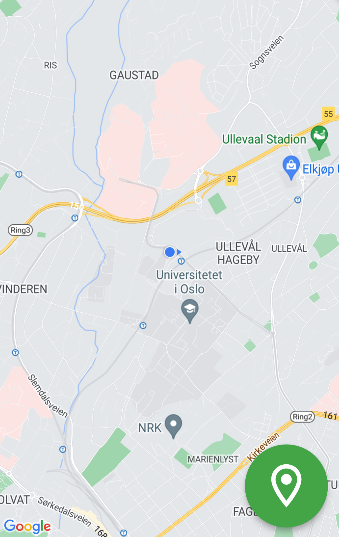
\includegraphics[width=\linewidth]{graphics/recording_off.png}
        \caption{Shows that the physical location recording is \emph{off} (green button)}
        \label{fig:recording_off}
    \end{minipage}
    \hfill
    \begin{minipage}[c]{0.34\linewidth}
        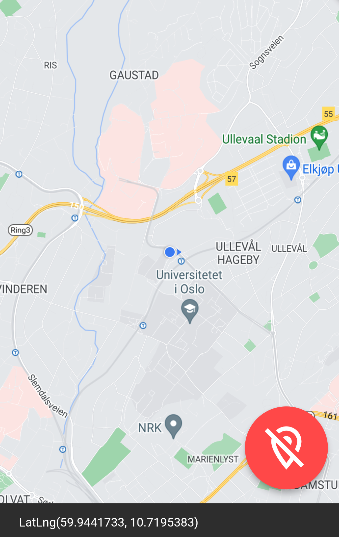
\includegraphics[width=\linewidth]{graphics/recording_on.png}
        \caption{Shows that the physical location recording is \emph{on} (red button)}
        \label{fig:recording_on}
    \end{minipage}
\end{figure}

We created a Maven project (a tool for managing the project) and used the object-oriented programming language Java for the server implementation. To let the server track many clients, we first assigned an ID to the client when it connected to the server which kept track of joining clients. The client received its assigned ID from the server which was later sent alongside the client's physical location as status update messages when pressing the button again. As this was an early adaptation, we implemented client-server communication over TCP (Transmission Control Protocol).

An asset model (ontology) of a simple building was also created, as shown in Figure \ref{fig:simple_building} (this time with coordinates as data properties which were "added" to individuals of the \verb|MovableEntity| class suggested in Section \ref{subsubsec:DynamicAssetModel}. We used Protégé to create the domain and exported it as an OWL document (file). This file was then accessed in a new SMOL program based on the background information in Section \ref{subsubsec:Technologies}, Section \ref{subsubsec:SMOL}, and from further analysis in Section \ref{subsubsec:StaticAndDynamicData}. 

To sum up, in the early version of the implementation a simple app was created to send sensor data (physical location from GPS-sensor in the devices as described in Section \ref{subsec:AppDevelopment}) to a server. Furthermore, the file containing information about a simple building domain was accessed in SMOL.


\subsection{Implemented solution}\label{subsec:ImplementedSolution}
Figure \ref{fig:components} shows the architectural components in the final implementation. More specifically, it illustrates the \textbf{Mobile Assets} in the \textbf{Physical Twin}, its \textbf{Digital Twin} based on a dynamic \textbf{Asset Model}, and the \textbf{Server} which enables the communication between the PT and DT both ways. In addition to this, the figure illustrates that the database \textbf{Firebase Realtime} acts as a channel between the \textbf{Physical Twin} and the \textbf{Server}, and that \textbf{InfluxDB Time Series} is used for storing the sensor data which \emph{can} be accessed from the \textbf{SMOL} program, as shown in the example function in Figure \ref{fig:access_time_series}.

In the following sections, we describe the architectural \emph{components} in the figure one by one based on the background information and the analysis, and by referencing the corresponding \emph{part} (Client, Server, Databases, or Semantic Digital Twin) in the structural requirements.

For further reference on how we setup SMOL to be used in \emph{this} thesis, see Section \ref{subsec:Setup}.

\subsubsection{Client}
A Flutter app was written in Dart, based on the background information of app development in industry in Section \ref{subsec:AppDevelopment}, and from the analysis of related technologies and their benefits in Section \ref{subsubsection:AppDevelopment}. From the paragraph about GDPR (General Data Protection Regulation) in Section \ref{subsec:AppDevelopment} and the requirement "Ask for permission to track the physical location of the device" we implemented location permissions. Section \ref{subsec:privacy} discusses privacy further. The map screen in the app was created with the wireframe shown in Figure \ref{fig:wireframe_app}. We did not bother implementing a login-screen because of the context of a crisis situation and due to the limited data stored in Firebase.

The source code of the app was structured into the following parts: 
\begin{itemize}
    \item \verb|main.dart| which initializes the app and Firebase
    \item \verb|map.dart| which contains code for the UI (User interface) in the app. This is done by rendering Flutter widgets.
    \item \verb|service.dart| accesses Firebase, and writes to, or reads from it.
    \item the model-class \verb|status.dart| is used to create status objects which are sent as JSON to Firebase in which it is stored as a JSON object, as described in Section \ref{subsec:Databases}.
\end{itemize}
We used the Google Maps SDK (Software Development Kit) in the implementation to integrate the map and its functions in the app, as described in Section \ref{subsec:AppDevelopment}.

Some of the requirements set forth in the structural requirements were already implemented in the earlier version of the app, such as "Client can choose to send its newest status (ID, latitude, longitude)" However, there are two requirements stating that we have to \emph{clearly} show when the recording function is off/on. In order to clearly show it for those that are color blind as well, the colors of the button changed to blue and red, respectively. Figure \ref{fig:color_theme} shows the final color theme, which is located in the previously mentioned file \verb|main.dart| and can be accessed from anywhere in the app. 

\begin{figure}[H]
    \centering
    \begin{minted}{dart}
final ThemeData _theme = ThemeData(
    colorScheme: ColorScheme.fromSwatch().copyWith(
        primary: const Color(0xFF2A3282),
        secondary: const Color(0xFFE81313),
    )
);
\end{minted}
    \caption{The color theme in the app}
    \label{fig:color_theme}
\end{figure}



The Dart code in Figure \ref{fig:location_toggle} shows the conditional rendering of the location recording button which uses the color theme above. Since the Flutter widgets are rendered and the color of the button was initially set, we had to keep track of the state to change the color of the button. This was done by adding new status messages to \verb|_messages| or emptying the list in \verb|setState(() { });|. The underscore as the leading character in \verb|_messages| means that the member is only visible in its class, much like using \verb|private| for members in Java. The code also shows the use of a ternary operator, which is syntactic sugar for the conditional operators \verb|if| and \verb|else|.
\begin{figure}[H]
    \centering
    \begin{minted}[breaklines]{dart}
    floatingActionButton: _messages.isEmpty ? FloatingActionButton.large (
        onPressed: () => _start(),
        backgroundColor: Theme.of(context).colorScheme.primary,
        child: const Icon(Icons.location_on_outlined, size: 60),
    ) : FloatingActionButton.large (
        onPressed: () => _stop(),
        backgroundColor: Theme.of(context).colorScheme.secondary,
        child: const Icon(Icons.location_off_outlined, size: 60)
    ),
    \end{minted}
    \caption{Rendering of the location recording button in the app}
    \label{fig:location_toggle}
\end{figure}

Furthermore, when recording of the physical location stops, the appropriate (endangered) clients are warned, as required in in the structured requirements. Firebase \emph{stores} the informed decisions, which the real-time database gets from the Digital Twin (DT) \emph{through} the server (as long as the DT has made a decision from sufficient information as analysed in Section \ref{subsubsec:FurtherDataSeparation}. Figure \ref{fig:safe_smartphone} and Figure \ref{fig:endangered_smartphone} show the conclusion of being \emph{safe} and \emph{endangered}, respectively.

\begin{figure}[H]
    \centering
    \begin{minipage}[c]{0.40\linewidth}
        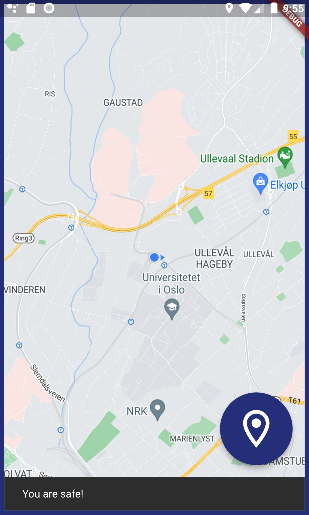
\includegraphics[width=\linewidth]{graphics/safe_smartphone.png}
        \caption{Shows that the mobile asset (smartphone) in the PT is \emph{safe} as concluded by the DT}
        \label{fig:safe_smartphone}
    \end{minipage}
    \hfill
    \begin{minipage}[c]{0.40\linewidth}
        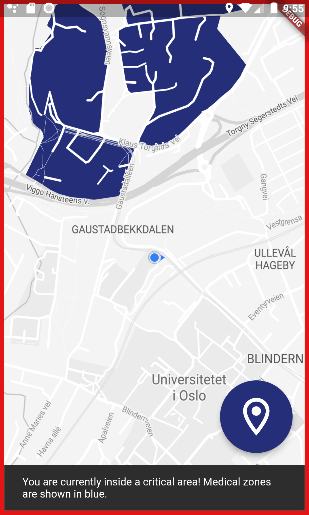
\includegraphics[width=\linewidth]{graphics/endangered_smartphone.png}
        \caption{Shows an \emph{endangered} smartphone from the informed decision to be inside a critical area, as concluded by the DT}
        \label{fig:endangered_smartphone}
    \end{minipage}
\end{figure}

\subsubsection{Server}
The main purpose of the server is to enable full communication both ways simultaneously between the PT and the DT. Sensor data from the PT are forwarded to the DT through InfluxDB, whilst informed decisions are forwarded to Firebase. This is done simultaneously in intervals by using threads. Thus the server enables seamless bidirectional data flow between the outermost architectural components in Figure \ref{fig:components}. The \emph{items} in the \emph{server}-part in the structural requirements in Section \ref{subsec:Requirements} support this. When the server runs, connections to Firebase and InfluxDB (time-series database) are first set up. Then the server forwards sensor data to the DT by sending the updated status of individual mobile assets in the PT to the time-series database, assuming there is sensor data in each run. The smartphones are also added to the asset model with their assigned IDs. Figure \ref{fig:server_get_sensor_data} shows the implemented solution to get updated sensor data from Firebase. Note that we had to implement a workaround because of the \verb|@Measurement|-annotation in the \verb|Data|-class, in order to create objects of it.

\begin{figure}
    \centering
    \begin{small}
    \begin{minted}[breaklines]{java}
public void getSensorData() {
    reference.addValueEventListener(new ValueEventListener() {
        @Override
        public void onDataChange(DataSnapshot dataSnapshot) {
            for (DataSnapshot snapshot : dataSnapshot.getChildren()) {
                String json = new Gson().toJson(snapshot.getValue(Object.class));
                Data data = new Gson().fromJson(json, Data.class);
                influxDB.insertDataPoint(data);
                System.out.println("Forwarded sensor data to DT!");
                try {
                    Owl.addIndividual(data);
                } catch (OWLOntologyCreationIOException e) {
                    e.printStackTrace();
                }
                hasSensorData = true;
            }
        }
        @Override
        public void onCancelled(DatabaseError databaseError) {
            System.out.println("Could not retrieve data from realtime database.");
        }
    });
}
    \end{minted}
    \end{small}
    \caption{Get updated sensor data from Firebase}
    \label{fig:server_get_sensor_data}
\end{figure}

Figure \ref{fig:server_forward_informed_decision} has a call to a function in the \verb|Owl|-class. The line \verb|Owl.addIndividual(data)| calls the function with the only parameter being the specific timestamped status message (data). In the function being called, we ensured the static data in the file (building.owl) written to was not affected by the data.


Figure \ref{fig:server_forward_informed_decision} shows how the informed decision from the DT is forwarded to Firebase.
\begin{figure}
    \centering
    \begin{small}
    \begin{minted}[breaklines]{java}
private void warnEndangeredClients(Map<String, String> results) {
    reference = FirebaseDatabase.getInstance().getReference("endangered");
    DatabaseReference.CompletionListener completionListener = (databaseError, databaseReference) ->
            System.out.println("Forwarded informed decision to PT!");
    reference.setValue(results, completionListener);
    reference.removeValue(completionListener);
}
    \end{minted}
    \end{small}
    \caption{Forward informed decision to PT through Firebase}
    \label{fig:server_forward_informed_decision}
\end{figure}


The server prepares to send sensor data to the time-series database whenever there are new clients in the PT, or when any of them has an updated physical location, by keeping a reference to the list of smartphones stored in Firebase. Whenever there is a single change in the referenced list, the server forward the sensor data of \emph{all} clients in it, so the DT gets can get the overall picture of the different locations at a specific point in time. Figure \ref{fig:insert_point} shows how a measurement point is inserted into InfluxDB. As can be seen in the figure, the programming language used is Java. A point is made from the model-class \verb|Data|. More specifically, the instance of the \verb|Data|-class is a timestamped status message.

\begin{figure}[H]
    \centering
    \begin{minted}{java}
public void insertDataPoint(Object object) {
    WriteApiBlocking writeApi = db.getWriteApiBlocking();
    writeApi.writeMeasurement(bucket, org, WritePrecision.MS, object);
}
    \end{minted}
    \caption{Inserting a measurement point (timestamped status message) into the Data-bucket in InfluxDB}
    \label{fig:insert_point}
\end{figure}

According to the structural requirements, the server should reload the asset model with clients that are currently tracked and access the generated knowledge graph from the DT. To reload the asset model, we used the exported OWL document (file) and put the file into the DT file structure (we later discuss how data can be stored, the reasons for using files, and the limitations to this in Section \ref{subsec:StoringData}, that the server accesses and writes to using the Java framework OWL API which is described in Section \ref{subsec:Reasoning}. Based on the background information of semantic technologies in Section \ref{subsubsec:Technologies}, and the example of adding \textbf{individuals} of \textbf{MovableEntity} to the asset model (ontology) in Section \ref{subsubsec:StaticAndDynamicData}, we created a function for adding data of a smartphone to the file. Before this, we tried to use Apache Jena to reload the asset model, but it could not write data in Turtle syntax to the asset model, and we suspect some compatibility issues with the Turtle syntax in the file exported from Protégé.

Apache Jena was used to access the endangered mobile assets in the knowledge graph which was generated from a combination of the knowledge base and the state of the SMOL program in the DT. More specifically, a model of the RDF graph was loaded, and the informed decisions were forwarded to Firebase to "close the loop" of the bidirectional flow of data between the PT and the DT, as shown in Figure \ref{fig:components}.

\subsubsection{Databases}
This section shortly describes how data is stored in Firebase and InfluxDB.
In Firebase, the assigned clients are stored as unstructured nodes (JSON objects) in the list \verb|mobiles|. As discovered in the analysis of technologies in Section \ref{subsubsection:Databases}, the number of nodes that can be stored are \emph{limitless}. The IDs of the endangered smartphones are also stored in a list, that is accessed by a function in \verb|service.dart| in the app. Time-series data is stored in InfluxDB in a bucket named \verb|Data|, in which there is sensor data that the SMOL program in the DT accesses. From this, the structural requirements regarding databases are met.


\subsubsection{Semantic Digital Twin}
From the background information of DTs in Section \ref{subsubsec:DigitalTwins} we created a digital twin, based on a dynamic asset model of a simple building, that handled mobile assets. The asset model had areas with predefined coordinates (latitude1, latitude2, longitude1, and longitude2) The DT and its parts were semantically enriched by using the semantic technologies presented in Technologies, as well as by using SMOL as an enabler of semantics from the analysis of it in Section \ref{subsubsec:SemanticDigitalTwins}. 

The \emph{semantic} digital twin was created in SMOL by using its core language illustrated in Section \ref{subsec:SMOL}. And by using the SMOL Interpreter (\verb|smol.jar|) in the file structure to read and execute the SMOL program. The SMOL program consists of two modular parts, namely: 
\begin{enumerate}
    \item \textbf{DS} (Digital Shadow) acts as a timestamped snapshot of a specific smartphone, as well as being used to access the newest sensor data, from the descriptions in Section \ref{subsubsec:FurtherDataSeparation}. It accesses the latest physical locations from a specified time ago. Based on the descriptions in Section \ref{subsec:Databases}, and from the example in Figure \ref{fig:access_time_series}, we accessed the updated sensor data in the DS. This can be seen in the function in Figure \ref{fig:DigitalShadowInflux}. Note that it looks like we get outdated sensor data (\textbf{first} added to the bucket), but we are actually getting the latest. When this was implemented there was no support for single-quote string delimiters in \verb|access|.
    \item \textbf{Digital Twin} is a digital representation of the PT. It accesses: 
    \begin{enumerate}
        \item the critical areas in a building domain defined in the asset model
        \item the smartphones by their IDs from the asset model
        \item the updated physical location of the smartphones from the asset model, based on a revised version of Figure \ref{fig:access_time_series}.
    \end{enumerate}
\end{enumerate}

\begin{figure}[H]
    \centering
    \begin{small}
    \begin{minted}[breaklines]{dart}
List<Double> getSmartphoneCoordinates()
    List<Double> coordinates = null;
    coordinates = access(
        "from(bucket: \"Data\")
            |> range(start: -20m)
            |> filter(fn: (r) => r[\"_measurement\"] == \"data\")
            |> filter(fn: (r) => r[\"_field\"] == \"latitude\" or r[\"_field\"] == \"longitude\")
            |> sort(columns: [\"_time\"], desc: true)
            |> unique(column: \"id\")
            |> aggregateWindow(every: 5m, fn: first, createEmpty: false)
            |> yield(name: \"first\")",
        INFLUXDB("influx.yml")
        );
    return coordinates;
end
    \end{minted}
    \end{small}
    \caption{Accessing the updated sensor data from InfluxDB}
    \label{fig:DigitalShadowInflux}
\end{figure}

From this, smartphone objects are created by combining the data as shown in Figure \ref{fig:smartphone_object} by matching the IDs accessed from InfluxDB and the smartphones in the asset model. The \emph{first four requirements} in the twin-part in the structural requirements in Section \ref{subsec:Requirements} are thus met. 

\begin{figure}[H]
    \centering
    \begin{minted}{dart}
MovableEntity smartphone = new MovableEntity(id, lat, long, False);
    \end{minted}
    \caption{Creating a smartphone object from the smartphone ID in the asset model, in combination with the corresponding updated coordinates from InfluxDB. \textbf{False} simply means the smartphone is not concluded to be endangered yet}
    \label{fig:smartphone_object}
\end{figure}

Referencing the requirement "Check if smartphones are inside any critical areas" we must understand what it \emph{means} before we can implement it. An example is described in Section \ref{subsubsec:RQ2}, where an informed decision can be made if the \emph{criteria} in the example evaluate to be true. The code implementation of it is shown in Figure \ref{fig:inside_critical_area}, where the function is located inside the Area-class. Meaning, we write \verb|area.containsPoint(lat, long)| to check if \verb|area| contains the smartphone with latitude (\verb|lat| and longitude \verb|long|).


\begin{figure}[H]
    \centering
    \begin{small}
    \begin{minted}[breaklines]{dart}
Boolean containsPoint(Double lat, Double long)
    Boolean inAnyLatitudeRange = ((lat >= this.latitude1) & (lat <= this.latitude2)) | ((lat >= this.latitude2) & (lat <= this.latitude1));
    Boolean inAnyLongitudeRange = ((long >= this.longitude1 & long <= this.longitude2)) | ((long >= this.longitude2) & (long <= this.longitude1));

    if (inAnyLatitudeRange & inAnyLongitudeRange) then
        return True;
    end
        
    return False;
end
    \end{minted}
    \end{small}
    \caption{Checking if a smartphone is inside a critical area based on coordinates, assuming they align}
    \label{fig:inside_critical_area}
\end{figure}

If the DT concludes that a smartphone \emph{is} inside \emph{any} of the critical areas which are accessed from the domain, the twin sets \verb|smartphone.endangered = True;| and adds the smartphone object to the specific area's list of endangered smartphones as a result, which is shown in Figure \ref{fig:add_endangered}. Note that what is shown in the figure is inside a while-loop for the context of the counter \textbf{j}.

\begin{figure}[H]
    \centering
    \begin{minted}[breaklines]{dart}
a = areas.get(j);
isInsideACriticalArea = a.containsPoint(lat, long);
if (isInsideACriticalArea) then
    smartphone.endangered = True;
    a.smartphones = new List<MovableEntity>(smartphone, a.smartphones);
end
    \end{minted}
    \caption{Automatically checking if a smartphone is inside a critical area. If the area contains its point (x, y), the smartphone is set to endangered, and is added to the list of the endangered smartphones for the specific area}
    \label{fig:add_endangered}
\end{figure}

Regarding the last requirements of this part, informational messages, such as examples of SPARQL queries, are shown in the REPL during the program execution. Figure \ref{fig:sparql_smol} show how we can \emph{manually} manually check which smartphones are inside a critical and thus are endangered, and the results (information about endangered smartphones). The querying is done in the SMOL REPL, which is started from the information in Section \ref{subsubsec:SMOLInterpreter}.

\begin{figure}[H]
    \centering
    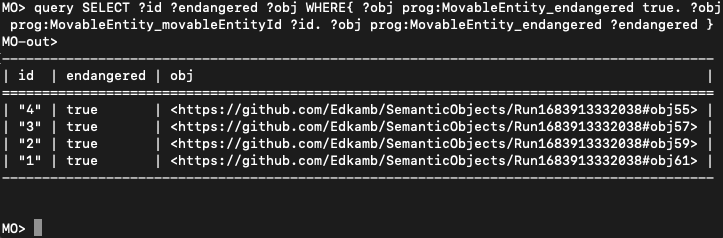
\includegraphics[scale=0.44]{graphics/sparql_smol}
    \caption{Querying with SPARQL}
    \label{fig:sparql_smol}
\end{figure}

The DT handles newly added smartphones to the asset model that don't have a physical location as well, and thus all requirements are met.

Lastly, Section \ref{subsubsec:SemanticDigitalTwins} describes the use of \verb|dump| in the REPL (Read-eval-print loop) to generate the knowledge graph, which the server uses by doing the following:
\begin{enumerate}
    \item Creates a \emph{model} of the knowledge graph with Apache Jena
    \item Reads the model
    \item Iterates over the resources (smartphones) in it
    \begin{itemize}
        \item If the smartphone is endangered, the ID of it is added to a list 
    \end{itemize}
    \item Adds the list of IDs to Firebase
\end{enumerate}

Clients in the PT then access Firebase, and are warned if they are in danger from the informed decision, which closes the loop.

\section{Evaluation}\label{sec:Evaluation}
This chapter evaluates the developed implementation in terms of which structural requirements in Section \ref{subsec:Requirements} are met from the analysis in this thesis in Chapter \ref{sec:Analysis}, and from performing various test runs in the following sections. We start by presenting the overall evaluation of the implementation according to the requirements. In the following section, we shortly describe how we set up SMOL to be used in the implementation. Then we provide test runs of the server automatically reloading the asset model, and of an operator manually editing the asset model by adding smartphones to it. Then we evaluate how long it takes to warn endangered clients of an informed decision. We also evaluate how the system scales with many heterogeneous smartphones, and plot the results in Data Explorer in InfluxDB.

The Structural requirements were divided into four parts, one for each of the \emph{main} architectural components shown in Figure \ref{fig:components}: \textbf{Client}, \textbf{Server}, \textbf{Databases (\textbf{Firebase Realtime} and \textbf{InfluxDB Time Series}}, and \textbf{Semantic Digital Twin}. 

The overall evaluation is shown in Table \ref{tab:overall_evaluation}:
\begin{small}
\begin{table}[H]
    \centering
    \begin{tabular}{|l|l|c|}
    \hline
    & \textbf{Requirement} & \textbf{Status} \\
    \hline
    \textbf{Client}\multirow{6}{0em} & Can choose to send its newest status (ID, latitude, longitude & \checkmark \\
    & Appropriate endangered clients are warned & \checkmark \\
    & Show appropriate in-app messages to the user & \checkmark \\
    & Ask for permission to track the physical location of the device & \checkmark \\
    & Clearly show when the physical location of the device is tracked & \checkmark \\
    & Clearly show when the physical location of the device is \emph{not} tracked & \checkmark \\
    \hline
    \textbf{Server}\multirow{5}{0em} & 1. Forward the sensor data to a time series database & \checkmark \\
    & 2. Forward the informed decisions to a real-time database & \checkmark \\
    & Should be possible to do \textbf{1.} and \textbf{2.} above at the same time & \checkmark \\
    & Reload asset model with tracked clients & \checkmark \\
    & Access and read the generated knowledge graph & \checkmark \\
    \hline
    \textbf{Databases} & \textbf{Firebase:} Store the ID and physical location of the clients & \checkmark \\
    & Store data about which clients the DT made an informed decision for & \checkmark \\
    & \textbf{InfluxDB:} Store the time series data & \checkmark \\
    \hline
    \textbf{Twin}\multirow{6}{0em} & 3. DS gets the newest sensor data from the time series database & \checkmark \\
    & 4. Access the smartphones in the asset model by their IDs & \checkmark \\
    & Create smartphone objects by combining data from \textbf{3.} and \textbf{4.} above & \checkmark \\
    & Access the critical areas from the asset model & \checkmark \\
    & Check if smartphones are inside any critical areas & \checkmark \\
    & Handle new smartphones that don’t have a physical location & \textbf{\texttimes} \\
    & Provide examples of SPARQL queries & \checkmark \\
    & Show informative messages in the REPL during program execution & \checkmark \\
    \hline
    \end{tabular}
    \caption{Overall evaluation of the structural requirements}
    \label{tab:overall_evaluation}
\end{table}
\end{small}


The only requirement that was not fully met, was that the DT should be able to handle any smartphones that didn't have a registered physical location. The SMOL program accesses the asset model and creates objects from all smartphones in it, but only adds the physical location to the smartphones that have their data in InfluxDB. However, there is no further support for adding the latitude and longitude to the objects. However, this is reflected in the knowledge graph, there is error handling in the SMOL program, and the REPL prints information regarding this. We also assumes that an operator \emph{knows} how to add smartphones to the asset model by either loading it into an ontology editor or use the template described in Section \ref{subsubsec:RQ1}.


\subsection{Setup of SMOL}\label{subsec:Setup}
To setup SMOL to use in the implementation in this thesis, we cloned the GitHub repository with
\newline 
\verb|git clone https://github.com/smolang/SemanticObjects.git|
\newline
Then we created jar-file, named \verb|smol.jar|, from the source code, and put the file in the created folder at the relative file path \verb|master/twin|. Then we navigated into it with \verb|cd master/twin| and used the SMOL interpreter (\verb|smol.jar|) as described in Section \ref{subsubsec:SMOLInterpreter}. A good and more general guide to using SMOL is publicly available\footnote{\url{https://github.com/smolang/SemanticObjects}}.

\subsection{Test runs}\label{subsec:test_runs}
When evaluating the implementation, it's important that we do it in a real-life environment. We are therefore performing the test runs on a public network with real physical devices. We will not evaluate in terms of performance in this section, as this is done in Section \ref{subsec:time_to_warn}. We instead provide a guide to using the implemented solution by describing what is going on, illustrating the running components, and examining it in terms of the requirements. It is a single test run of bidirectional data flow.

Before we started the test runs, we emptied the databases, removed smartphones from the asset model, ran the SMOL program, and generated the knowledge graph. To set up the digital twin, we moved inside the \verb|twin|-directory, containing the file \verb|smol.jar|, in the terminal, and then used:

\begin{small}
\begin{lstlisting}[breaklines]
    java -jar smol.jar -d http://www.semanticweb.org/oscarlr/ontologies/2023/2/building# -b building.owl
\end{lstlisting}
\end{small}
From this, the REPL was ready to use, and the knowledge graph reflected that there were \emph{no} tracked smartphones.

\subsubsection{Automatically reloading asset model}
As the scene was set, we first started the server. Then we ran the SMOL program in the DT, and as expected, there were no time-series data, nor any detected clients, as no smartphones had sent their physical location.
We pressed the button shown in the map in the app in Figure \ref{fig:safe_smartphone}. The server is checking if there is any sensor data to forward to the DT (or whenever there is a change in the document by keeping the reference in the server code) in intervals, and if there is an informed decision that should be forwarded to the PT. As the smartphone had sent its physical location, it was assigned an ID, added to Firebase, which was detected by the server, as shown in Figure \ref{fig:detected_by_server}.

\begin{figure}[H]
    \centering
    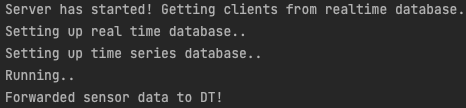
\includegraphics[scale=0.50]{graphics/detected_by_server.png}
    \caption{Shows the server detecting a smartphone}
    \label{fig:detected_by_server}
\end{figure}

Based on the background information in Section \ref{subsec:AssetModel}, the server added the smartphone individual to the asset model according to the template described in Section \ref{subsubsec:RQ1}.

Whenever the server notices a change in the physical data in Firebase (or in timed intervals), all physical location data is timestamped and sent to InfluxDB. When the DS in the twin gets this data, the DT uses it to get a picture of the physical location of the smartphones at a specific point in time. Figure \ref{fig:influx} shows the time-series data in the graph view in InfluxDB. We can see that the server constantly forwards the sensor data. This is also the basis for \textbf{InfluxDB} in Figure \ref{fig:static_dynamic_asset_model}.

\begin{figure}[H]
    \centering
    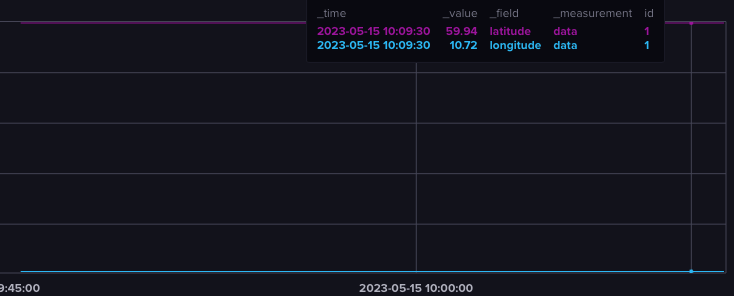
\includegraphics[scale=0.40]{graphics/influx.png}
    \caption{Time-series data in InfluxDB}
    \label{fig:influx}
\end{figure}

We closed and reopened the app twice to get new IDs whilst moving around, and checked the different physical locations in the map view in the time-series database, which is illustrated in Figure \ref{fig:influx_map}. In the figure, different IDs have different colors. We also illustrate that the smartphone with ID 1 (blue) have multiple tracked physical locations. The information window is off the smartphone with ID 2 (red).

\begin{figure}[H]
    \centering
    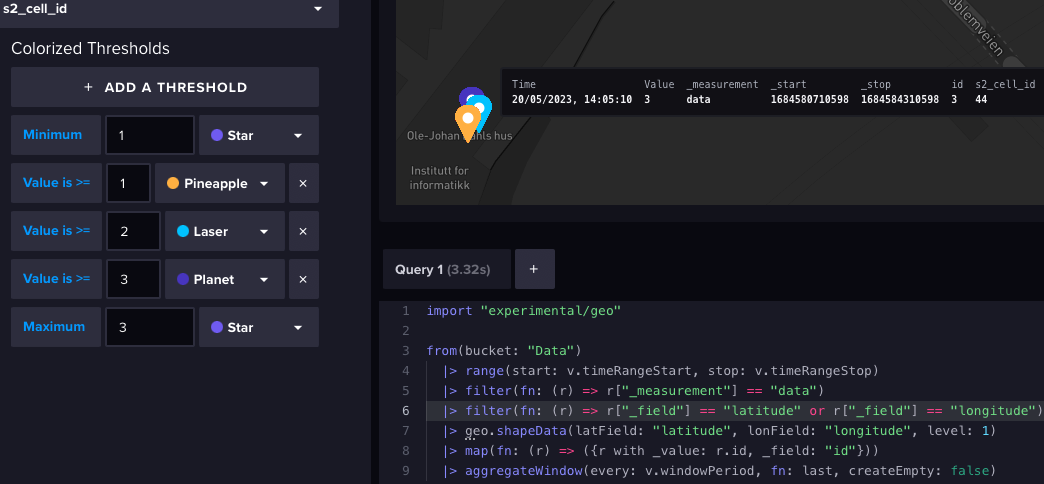
\includegraphics[scale=0.50]{graphics/influx_map.png}
    \caption{Time-series data represented in a map in InfluxDB from using a Flux query}
    \label{fig:influx_map}
\end{figure}

After this we ran the SMOL program with \verb|reada main.smol|, and the DT sent the informed decision that all of the clients were inside the critical area IFI. We can also see that all smartphones in the domain have a physical location in "\textbf{4. All smartphone(s) in the domain have a physical location}". A SPARQL query was also run in the REPL with results in which the smartphones are set to endangered.

The last thing \emph{we} had to do in the REPL was to use the \verb|dump| to generate the knowledge graph, which the server later read from. The informed decision was forwarded to the PT. The result from this was that the individual clients were warned in the app when they pressed the button, as shown in Figure \ref{fig:endangered_smartphone}.

\begin{figure}[H]
    \centering
    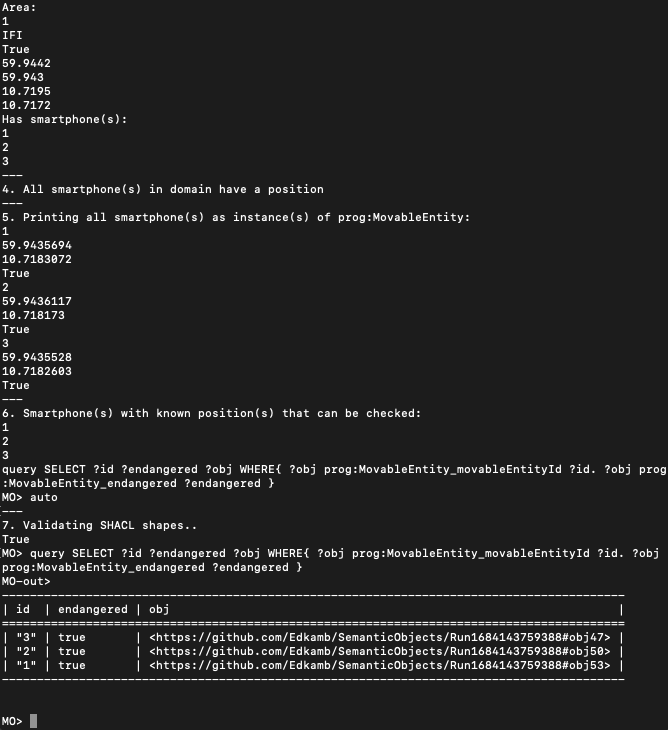
\includegraphics[scale=0.50]{graphics/digital_twin_repl.png}
    \caption{Shows the informative messages in the REPL from running the SMOL program in the DT}
    \label{fig:digital_twin_repl}
\end{figure}


 
\subsubsection{Manually adding smartphones}
Now we will manually add smartphones to the asset model by using the previous test run as a basis. The ideal scenario, taking into account what is stated in Chapter \ref{sec:Evaluation} regarding the requirement that was not met, the SMOL program should identify the smartphones with no physical location and the knowledge graph should reflect this. We use the description of manually adding it at the end of Section \ref{subsubsec:StaticAndDynamicData}. 

We stop the server, as it is updating the asset model in intervals, and it does not have to be started again. We also have to \verb|exit| the REPL, load the asset model again and execute the program. 
The result is that the print "\textbf{4. All smartphone(s) in domain have a physical location}" in Figure \ref{fig:digital_twin_repl} is replaced with what is shown in Figure \ref{fig:manually_adding_smartphone}.

\begin{figure}
    \centering
    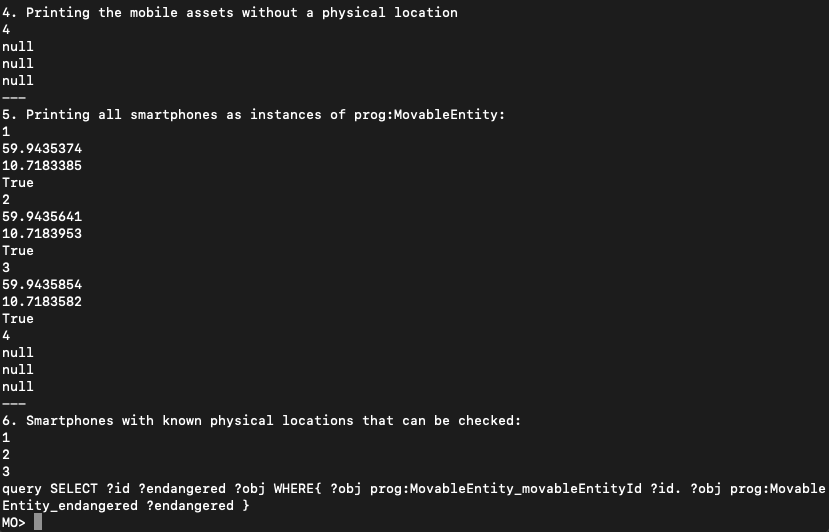
\includegraphics[scale=0.70]{graphics/manually_adding_smartphone.png}
    \caption{Printing any smartphones without a physical location}
    \label{fig:manually_adding_smartphone}
\end{figure}

We also validate SHACL shapes (described in Section \ref{subsubsec:Technologies}), which evaluates to true. We then skip the breakpoint in the program with \verb|auto|, generating the knowledge graph in which the data of the added smartphone is.


\subsection{How fast can we warn?}\label{subsec:time_to_warn}
In this section, we are evaluating the implementation in terms of how it performs in a realistic setting. Although not the main focus of this thesis, as we are to formalize knowledge, it is nonetheless interesting to take a look at. More specifically we are presenting how long it takes to warn an endangered smartphone, concluded by the DT.  
This evaluation, as well as the previous test runs, was performed on a MacBook Air with an M1 (2020) chip with 8 cores, and 8GB of RAM. We are again testing with physical devices over a public network as described in Section \ref{subsec:test_runs}.

The architecture shown in Figure \ref{fig:components} shows the bidirectional flow of data, namely sensor data sent from the PT, and informed decisions sent from the DT. This section evaluates how fast we can warn a specific client with ID. The elapsed time will be presented as the \emph{median} of ten runs, because the results may fluctuate due to the server reading the knowledge graph in intervals, and because it may take some time to generate the knowledge graph in SMOL. Before each run, The REPL is exited, and the asset model is loaded. We are manually using commands, first to load the asset model, then reading and executing the SMOL program at the same time with \verb|reada main.smol|. We are also typing \verb|auto|, and lastly dumping to the knowledge graph in each run. Then we wait for the server forward the informed decision. This time we are however not emptying the databases for a more realistic simulation. Also, because of the way the IDs are assigned, the appropriate clients will be warned.

An ideal approach in terms of performance at the expense of ensuring formalized knowledge would have been to read from the asset model directly from the server. The DT has to conclude that some smartphones are inside a critical area and set them to endangered, and writing to the asset model in the SMOL program is currently not supported. This means that the time it takes to warn clients depends on the time it takes to generate the knowledge graph, as well as use the REPL.

The elapsed time is evaluated by subtracting the end time (stops recording physical location) from the start time (starts recording physical location) in the app. Table \ref{tab:time_manual_work} shows the runs listed in chronological order.
\begin{table}[H]
    \centering
    \begin{tabular}{|c|c|}
        \hline
        \textbf{Run} & \textbf{Elapsed time in seconds} \\
        \hline
         1 & 15.304 \\ 
         2 & 17.143 \\ 
         3 & 19.574 \\
         4 & 18.939 \\
         5 & 18.847 \\
         6 & 19.992 \\
         7 & 17.569 \\ 
         8 & 17.732 \\ 
         9 & 17.197 \\ 
         10 & 17.447 \\
         \hline
         \textbf{Median time} & \textbf{17.732 seconds} \\
         \hline
    \end{tabular}
    \caption{Median time of sending sensor data to DT, sending the informed decision back to PT in which users are warned in the app}
    \label{tab:time_manual_work}
\end{table}


\subsection{Many smartphones}
In this section, we are evaluating in terms of number of smartphones. Since we don't have access to that many heterogeneous smartphones in the literal sense, we will instead conduct the experiment with one physical device running the app. We can test for scaling, but not for heterogeneity, but this  We will be walking around at IFI toggling the recording button on and off. 

We will edit the source code a little to ensure a new ID is assigned every time the physical location is sent from the smartphone, meaning we are able to simulate many smartphones. The problem with this, however, is the trade-off in terms of performance compared to the ideal scenario. By using different physical devices the performance would be better since we are not constantly sending the updated physical location to Firebase and re-rendering the UI in \emph{one} app. Taking all this into account, when the server gets the sensor data, there will not be much of a difference between this scenario and an ideal scenario.

Then after we have gathered the initial data which is stored in Firebase, we will start the server and look at how the system scales. Coordinates of 150 smartphones were added to Firebase, and then written to the asset model when the server was started. The SMOL program executed in almost no time, although we had to wait for the asset model to be fully written with IDs according to the IDs in InfluxDB.

The following Flux query was used on the time series data in InfluxDB by using the import:
\begin{small}
\begin{minted}[breaklines]{dart}
import "experimental/geo"

from(bucket: "Data")
  |> range(start: v.timeRangeStart, stop: v.timeRangeStop)
  |> filter(fn: (r) => r["_measurement"] == "data")
  |> filter(fn: (r) => r["_field"] == "latitude" or r["_field"] == "longitude")
  |> geo.shapeData(latField: "latitude", lonField: "longitude", level: 1)
  |> map(fn: (r) => ({r with _value: r.id, _field: "id"}))
  |> aggregateWindow(every: v.windowPeriod, fn: last, createEmpty: false)
\end{minted}
\end{small}

Figure \ref{fig:150_smartphones} shows the physical locations in the map view and that the Flux query above was used. Since we sent from one physical device this time, the pins have the same color with the only exception of the pin of a smartphone with ID 150 which is in purple (although hard to see). The information window in the figure is shown by hovering over this specific smartphone.


\begin{figure}[H]
    \centering
    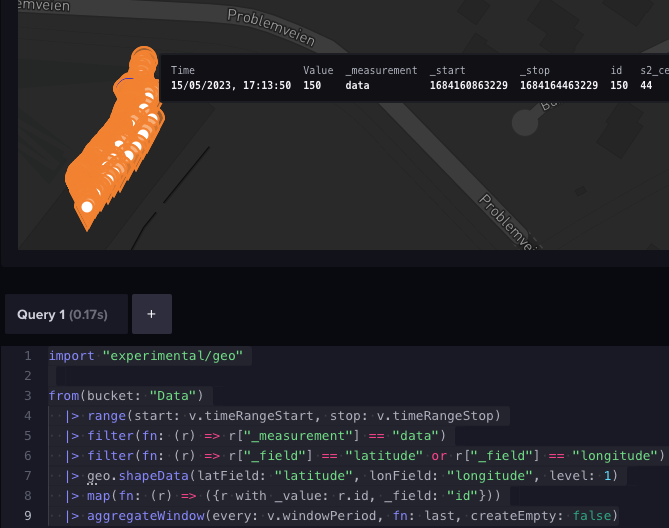
\includegraphics[scale=0.42]{graphics/150_smartphones.png}
    \caption{The result from simulating 150 smartphones}
    \label{fig:150_smartphones}
\end{figure}

Keeping this figure in mind as the basis for a PT (IFI) with mobile assets in it, we will now check manually with a SPARQL query which of the smartphones should be inside it and are thus endangered, concluded by the DT. The asset model contains IFI as a critical area.
We will now do various simple checks with SPARQL queries in the REPL, to understand if any smartphones in the PT are endangered. First, we can get information about the IFI as a critical area with:
\newline
\begin{small}
\verb|query SELECT ?id ?obj WHERE{?obj prog:Area_name "IFI". ?obj prog:Area_areaId id}| 
\end{small}

Then we check which smartphones are concluded by the DT to be inside IFI, and are thus \emph{endangered}, by running the SPARQL query:
\newline
\begin{small}
\verb|query SELECT ?obj WHERE{?obj prog:MovableEntity_endangered true}|
\end{small}

This resulted in all 150 smartphones being endangered. From this, the DT is evaluated to be a digital representation of the PT.

\newpage
\section{Discussion}\label{sec:Discussion}
In this chapter, we look at the discoveries in this thesis and compare them to other existing theories and results. Along the way, we discuss limitations with what was implemented and alternatives that could deal with them. In the last section, we discuss the implementation more in-depth.

\subsection{Dynamic data}\label{subsec:DiscussDynamicData}
In this thesis, we presented a way to separate data, mainly the two extremes: static data of building infrastructure, and the physical location of smartphones as dynamic data. However, this depends on the server being able to add the sensor data to InfluxDB fast enough to differentiate it from other data that may be considered static, but also because data of static building infrastructure is only static if it is not modified. In this thesis, \emph{how} dynamic data is to what extent it changes through time. From this, an alternative is presented to illustrate more shades of blue and red in Figure \ref{fig:dynamic_arrow}. In this figure, we can see that we \emph{can} put \textbf{Building Infrastructure} as more static compared to \textbf{Physical Location}, but we don't \emph{have} to. Also meaning, the ordering of the documents above the arrow in the figure can be reordered in any way, and removed for that matter.

\begin{figure}[H]
    \centering
    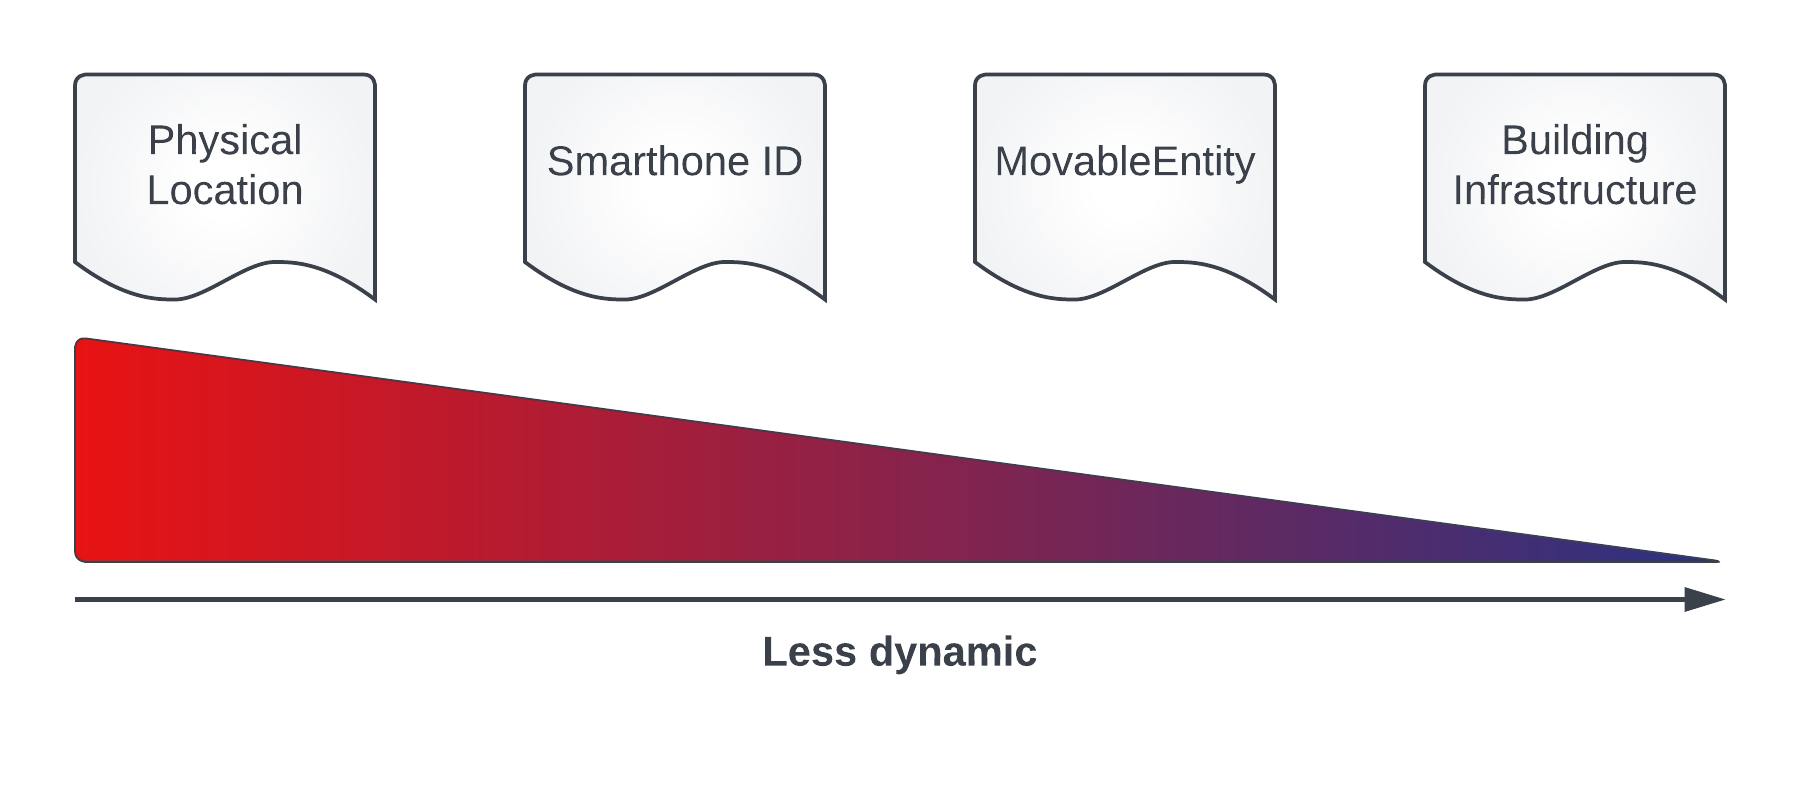
\includegraphics[scale=0.16]{graphics/dynamic_arrow.png}
    \caption{This figure shows to what degree data could be considered dynamic}
    \label{fig:dynamic_arrow}
\end{figure}


\subsection{Data in the twin}\label{subsec:StoringData}
In the digital twin, we are storing data in files. The asset model is stored as the file (\verb|building.owl|), and the knowledge graph is stored in a file named (\verb|output.ttl|). The proposals from \citeauthor{waszak_let_2022} and \citeauthor{gulnes_graph-based_2020} provide solutions for storing data in graph databases, such as Neo4j. This allows for better structuring of the data, as well as better representations of the graphs. Due to this, there are limitations with the implementation in this thesis as we store RDF graphs in files. Storing and exporting RDF graphs (such as the data in the asset model) to a graph database like Neo4j would be ideal. Instead of updating a graph database with the updated knowledge graph, produced from the combination of the program state and knowledge base, it could be considered feasible to store it in the twin. However, this means the server must know where the file is located in the local structure, as well as be able to access it. A better solution would therefore be to store it in a graph database and then get this data over the internet, assuming we want a clear architectural separation of the server and the twin. The architecture in this thesis is already very extensive and therefore we had to make some choices on what to focus on.


\subsection{Client-server communication}\label{subsec:ClientServerCommunication}
We looked at web sockets and FastAPI\footnote{\url{https://github.com/tiangolo/fastapi}} to decide how the clients should communicate with the server. Although another solution \cite{waszak_let_2022} uses FastAPI in architectural interconnection (not between client and server in this case), Firebase real-time database was chosen as a channel because of previous experience with integrating it with the cross-platform framework Flutter, and due to intuitively being able to modify data there. The difference between Firebase and FastAPI in terms of performance remains unclear, however, but as Firebase is based on web sockets, its use was justified. Lastly, the choice meant we let clients use some parts of the app without the server running, and updating the database with offline-data when online again.

\subsection{Dimensions and areas}
Figure \ref{fig:simple_building} shows a simple building consisting of different built components. In this figure, the built components (coordinates are in two dimensions, and are not built components), are in one dimension. One dimension means we can have a length or a width or a height. We later describe how we can create an ontology from this in Figure \ref{fig:building_ontology}. It shows that a Room individual \emph{can} be left or right of another Room individual. Because of this, although there is no ordering of descriptive names of \emph{one} dimension, it would be easiest to understand it as a length, which is also the convention to be used before 2. width and 3. height.
\newpage

\subsection{Privacy}\label{subsec:privacy}
Privacy is protected as much as possible in the implementation due to privacy concerns in tracking systems, especially in recent years. Data that can be used to identify an individual person is \emph{personal data} \cite{noauthor_gdpr_nodate, noauthor_hva_nodate}. We implemented such that the personal data now is \emph{pseudoanonymous} as well. This was done by assigning a new ID to the client every time the app was restarted as we don't need to permanently assign them. Only the ID and physical location are stored in Firebase, whilst the sensor data is stored for a maximum of thirty days in InfluxDB. More specifically, in Firebase endangered clients are stored by ID only, whilst IDs and the updated latitude and longitude coordinates are stored for the assigned clients. Note that there is no information on \emph{when} the data was collected as this is handled by the server when writing to the real-time database.


Pseudoanonymous data still qualifies as personal data under GDPR (General Data Protection Registration) \cite{noauthor_pseudonymous_nodate}. The data is not anonymous as the data is location dependent, and so movement pattern recognition can be used to correlate the data, and thus identify the individual data subjects (individuals).

The paragraph describing privacy in Section \ref{subsec:AppDevelopment} states that no personal data should be collected without the permission of the user (data subject). Because of this, the implemented app requests the data subject for permission to access the physical location of the device running it. We realize that to protect data even further, the specific purpose for data collection should be specified.


\subsection{Further discussion of implementation}
An alternative to the implemented digital twin (DT) is to make it wait a little while after it makes the informed decision and before it is sent to the physical counterpart, in which the smartphones are individually warned. One possible solution is to conclude that the user has not moved for a little while inside the critical area before the DT warns it. This is a limitation in this implementation as the user may have moved outside the critical area, meaning the informed decision could be misinforming for the user.

The server reads from the knowledge graph and not the asset model.
There is a limitation to how fast appropriate clients can be warned due to this, as described in Section \ref{subsec:time_to_warn}. This is because the server accesses the endangered smartphones from the knowledge graph, which has to be manually generated in SMOL by using the \verb|dump| command in the REPL, as described in Section \ref{subsubsec:SMOLInterpreter}. We could warn the clients faster if the server read from the asset model but at the expense of \emph{ensuring} formalized knowledge. This could be implemented by adding the physical location of the smartphones to the asset model from the SMOL program after smartphone objects are created, which the server would then access. But, this is currently not possible in SMOL. The server should however not add the physical locations to the asset model because a time-series database should be used for this, which is accessed in the SMOL. By doing this, it would mean a \emph{fully} automatic system as long as the server is running, and the SMOL program executes.

In the server, when writing to the asset model, or when reading from the generated knowledge graph, there is no reasoning done. As this could be considered a limitation, we should preferably also reason with the inbuilt tools from Apache Jena and OWL API. Instead, we made sure that dynamic data did not affect the static data when writing to the OWL document. We did however use the reasoner tool HermiT manually in Protégé from the background information in Section \ref{subsec:Reasoning} and in Figure \ref{fig:hermit_in_protege}, as well as automatically from SMOL, which showed consistency. And as the server queries what is already consistent, it was deemed unnecessary to reason further.

\newpage
\section{Conclusion and further work}\label{sec:Conclusion}
This chapter first summarizes the thesis research, and present the contributions in the light of it. Then we suggest examples of other directions to take in the future by using this thesis as a basis.

\subsection{Summary}
Recent years have seen a great increase in number of smartphone users. Smartphones are heterogeneous by nature, are important resources for a company, and can change at any time. Creating building domains with BIM (Building Information Modeling) is costly, as well as expensive to maintain, as movable assets change.  

Until now, a system for tracking mobile assets that had a semantic digital twin (DT) based on a dynamic asset model, did not exist. We also made it extensible by letting operators edit the asset model, and easily maintain it in an ontology editor such as Protégé. In addition to this, the implementation ensures static data (building infrastructure) is not affected by dynamic data (physical location of smartphones), and they are therefore separated. Furthermore, nor is the analysis of what a critical area \emph{is} affected by the dynamic snapshots in the twin. By using semantic technologies we have semantically enriched the DT, and formalized the knowledge of the mobile assets in it, which is ensured when the server reads the knowledge graph.

\subsection{Contributions}
From the research in this thesis, we developed a proof-of-concept implementation. It fully met all of the structural requirements as presented in Table \ref{tab:overall_evaluation}, apart from one that was only met partly. It was also evaluated from different different test runs, in terms of seamless bidirectional data flow, automatic reloading of the asset model, and extensibility. We also conducted an experiment to see how the DT scales with many smartphones in it (we did not try further than 150 mobile assets).

In light of the research and developing the final implementation, we will now address the research questions (RQ1, RQ2, RQ3), and then the hypothesis (H).

RQ1 asked, "How to create a dynamic asset model of a simple building that is also
extensible?". 
We started with the background information on asset models and their benefits compared to other modeling tools. Then an ontology of a simple building was created, which was also extended in the final implementation to support 2D areas. We also analyzed further what a \emph{dynamic} asset model entails in Section \ref{subsubsec:DynamicAssetModel}. All of this, but not limited to, resulted in an implementation that supports the research question. This was also evaluated to be the case.

RQ2 asked, "How to enable bidirectional data flow between the PT and DT, such that
the digital twin gets updated sensor data from mobile devices and sends
informed decisions back?".
From the background information on digital twins, as well as the realized architecture shown in Figure \ref{fig:components}, we were able to implement seamless coupled communication between the PT and the DT. From the evaluation of the app, appropriate clients are also warned, as shown in Figure \ref{fig:endangered_smartphone}.

RQ3 asked, "How to separate dynamic data (smartphone’s physical location) from
static data (building infrastructure) in the asset model?". There was in-depth analysis of this with illustrative examples in Chapter \ref{sec:Analysis}, and it was also discussed further in Section \ref{subsec:DiscussDynamicData}. The evaluation of the proposed implementation resulted in static data not being affected by dynamic data. This was also kept in mind when reloading the asset model with OWL API in ther server implementation. Also, there was further modularity in the code which separated the static analysis from the dynamic snapshots in the twin. 

\begin{itemize}
    \item[\textbf{H:}] We can handle mobile assets in a semantic digital twin with the use of a dynamic asset model of a simple building, in which dynamic data (smartphone's physical location) is automatically updated by a server and separated from static data (existing building infrastructure), and informed decisions are sent back to the physical twin.
\end{itemize}
Since all of the research questions guiding the problem statement have been answered, we will now answer to the hypothesis above. We have demonstrated that we have handled mobile assets in a digital twin, but not only by answering to the research questions. Although there were challenges along the way, and things that could have been done differently (such as letting newly added smartphones be tracked as well), we solved what we initially thought was possible.

\subsection{Further work}
There is further work that can be done by using what is described in this thesis. We will not explain this in too much detail as we want to leave it up to someone else to go in the direction \emph{they} want. But, we hope the proposed implementation from the research in this thesis, will be valuable in future endeavors.

\begin{itemize}
    \item \textbf{SMOL as an in-development research language:} Writing \emph{to} InfluxDB from SMOL is currently not possible, and so further work can be done with this, or with the proposed implementation itself, to get the physical location of the \emph{newly added smartphones} in the asset model and track their physical location as well. Alternatively, by adding the physical locations of the smartphones to the asset model, we can automatically warn endangered smartphones much faster at the expense of formalized knowledge.
    \item \textbf{Accuracy of physical location:} We have not focused on the accuracy of the physical locations as this has been researched extensively already, and we refused to open the door. It could be interesting to look at how accurate the sensor data from different heterogeneous smartphones and GPS' are, as well as check how this is reflected when the critical areas get comparably smaller.
    \item \textbf{3D:} We only support two dimensions in this thesis, and so further work could be done by adding support for a third dimension, e.g. height. An obvious limitation of this thesis is two rooms (one critical and one not) at different levels with the same latitude and longitude coordinates. Adding support for altitude should not be very hard by using the work in this thesis.
    \item \textbf{Point-in-polygon and Mercator projection:} Since we are only using square areas where we assume the coordinates align, we could not only use the point-in-polygon problem and check if smartphones are inside critical polygon areas. Further work could also be done with Mercator projection, because projecting the areas in this thesis on a map results in other shapes.
    \item \textbf{Proximity detection:} Further work could be done by checking how close smartphones are to other smartphones in the domain, and getting informed decisions from \emph{other clients} directly, effectively warning much faster. It should not come at the expense of privacy, however, as it should be protected as much as possible. We could also further check how close smartphones are to building infrastructure.
    \item \textbf{Anomaly detection:}: Further work on anomaly detection could be done which could be of great value. An example is if the movement pattern of a smartphone abruptly, and unrealistically, changes compared to the previous behavior. And if it is concluded to be suspicious by e.g. the digital twin, what should then be done?
    \item \textbf{Statistics} The work in this thesis can be used by, or improved by, other disciplines, such as Statistics. It could be interesting to create statistics on the movement of mobile assets through time.
    \item \textbf{Evaluation:} It could be interesting to evaluate how the RDF graph produced from the asset model, or the knowledge graph for that matter, changes through time, and to actually evaluate to what extent data is dynamic.
\end{itemize}

\newpage
\printbibliography


\end{document}